\documentclass[11pt,a4paper]{article}
\usepackage[utf8]{inputenc}
\usepackage[T1]{fontenc}
\usepackage[margin=22mm]{geometry}
\usepackage{amsmath,amssymb,booktabs,graphicx,hyperref,natbib,array,xcolor}
\title{When Online Mandi Prices Mislead: A Leak-Free Replay and Zero-Parameter Risk-Aware Dispatch Rules on Public Indian Wholesale Data}
\author{Aditya Sharma \\ Shoolini University, Solan, Himachal Pradesh, India}
\date{Revision v6 --- Cleanroom Reproducible Exploratory Audit}
\begin{document}
\maketitle

\begin{abstract}
Whether wholesale spreads on India's AGMARKNET portal survive transit hinges on how unobserved arrival-day blanks are interpreted. Under closed-yard sequential settlement (\texttt{div = 1.5} turn-back when a commodity is absent), chasing lagged spreads above \texttt{Rs.\,100/qtl} loses money on \textbf{\texttt{45.21\%}} of trips (\texttt{N = 58,676}, \texttt{1 June 2025--8 April 2026}, worst-10\% shortfall \texttt{ES10 -Rs.\,641.26/qtl}); under an open-yard Missing-At-Random (MAR) counterfactual assuming blanks cleared at lagged prices, road-adjusted dispatch (\texttt{B2\_age\_matched}) earns \texttt{+Rs.\,102.58/qtl} higher mean than zero-parameter dispatch (\texttt{Safe\_EV\_Sunk\_m0}).

Auditing six states and four crops (\texttt{178} markets; \texttt{42} HP apple yards) under a strict \texttt{<= t - 1} firewall, we evaluate three zero-hyperparameter rules needing no machine learning or tuning: \textbf{\texttt{Safe\_EV\_Sunk\_m0}} ($p_{\text{dow}} G_{\text{1SD}} > F_{\text{road}}$), settlement-matched \textbf{\texttt{Safe\_EV\_Phys\_m0}} (\texttt{1.5F}), and calculator rule \textbf{\texttt{RT\_2F\_Min\_m0}} ($p_{\min} G > 2 F_{\text{road}}$). Across \texttt{R = 5,000} cluster bootstraps (three market clusterings; 1-, 2-, 4-week blocks), \textbf{\texttt{Safe\_EV\_Sunk\_m0}} (\texttt{63.27\%} dispatch) attains \texttt{Rs.\,465.59/qtl} mean (\texttt{+Rs.\,32.03} vs \texttt{B2}, \texttt{p\_holm\_2s = 0.0028--0.0436}), \texttt{14.93\%} losses (\texttt{-11.79 pp}), and \textbf{\texttt{ES10 -Rs.\,344.09/qtl}} (\texttt{+Rs.\,181.17} vs \texttt{B2}; \texttt{Safe\_EV\_Phys\_m0} \texttt{+Rs.\,191.69}; \textbf{\texttt{RT\_2F\_Min\_m0}} Mean \texttt{Rs.\,478.38}, \texttt{+Rs.\,44.82}; tail/loss/\texttt{RT}-mean \texttt{p\_holm\_2s = 0.0024}). Gains persist on a fresh \texttt{2024}-only \texttt{171}-market rebuild (\texttt{N = 57,634}), realized ERA5 arrival-weather settlement (\texttt{+Rs.\,190.43} \texttt{ES10}), an \texttt{88,014}-episode unconditional panel, and all six states vs \texttt{B2} (break-even requires silent trips \texttt{+Rs.\,328.37/qtl} above turn-back; \texttt{23.79\%} MAR share). HP apples still lose on \texttt{41.38\%} of dispatches. These rules act strictly as a 6 a.m. alert filter ahead of trader calls; post-Stage-I results remain exploratory (\texttt{make reproduce}).
\end{abstract}

\section{Three Research Questions and Honest Methodological Scope}

Indian wholesale agricultural markets (\textit{mandis}) publish daily minimum, modal, and maximum prices by variety on AGMARKNET. While digital price dissemination can narrow spatial dispersion when market frictions are low \cite{jensen2007digital,goyal2010information}, empirical evidence across rural India and developing economies shows that raw price portals frequently fail to translate into realized arbitrage \cite{fafchamps2012sms,courtois2015farmer,mitra2018asymmetric,chatterjee2023market}. Four operational mechanisms separate a screen spread from realized net gain:

\begin{enumerate}
  \item \textbf{Decision-Time Reporting Lag:} At 6 a.m. dispatch time $t$---when FPO managers decide whether to load a truck or suppress a portal alert---same-day auction prices have not cleared, and thinner yards publish intermittently (\texttt{1..7} days late).
  \item \textbf{Transfer Costs, Destination Statutory Fees, and Biological Decay:} Road freight, single-lane hill terrain, out-of-district APMC seller fees levied on destination auction value, and ambient transit spoilage erode gross price gaps \cite{baulch1997transfer,nabcons2022phl}.
  \item \textbf{Auction Volatility and Arrival Execution Risk:} A single elevated lagged modal quote at a volatile market (\texttt{dest\_price\_cv\_28d}) frequently reverts by arrival day $t + \tau$, and an empty arrival board (\texttt{settle\_any\_min\_dw = NaN}) indicates no recorded commodity trade in the public portal \cite{deka2026missing}.
  \item \textbf{Role of Automated Triage vs Live Trader Confirmation:} Farmers dispatching a 30-quintal load normally verify live yard activity through a 30-second phone call to a destination \textit{arhtiya} (commission agent) \cite{jensen2007digital,ziegler2019fresh}. Automated dispatch scoring operates strictly as an \textbf{upstream 6 a.m. alert-triage filter} helping FPO coordinators prioritize promising corridors and suppress noisy alerts before dialing traders, rather than replacing phone verification.
\end{enumerate}

We address three research questions across six Indian states (Gujarat, Himachal Pradesh, Karnataka, Madhya Pradesh, Maharashtra, Uttar Pradesh) and four crops (Onion, Potato, Tomato, Apple):

\begin{itemize}
  \item \textbf{RQ1 (Screen-Chasing Loss Incidence and Settlement Realism):} Under a strict \texttt{<= t - 1} chronological firewall and non-anticipative sequential arrival settlement, how often do attractive lagged portal spreads (\texttt{> Rs.\,100/qtl}) lose money, and how strongly do 3-day hindsight settlement and ex-post day-$t$ origin conditioning distort observed risk?
  \item \textbf{RQ2 (Zero-Parameter Expected-Value Rules vs Equal-Age Baselines and Tuned Heuristics):} On identical Top-5 candidate menus and equal quote ages (\texttt{1..3} days), can threshold-free, zero-hyperparameter rules (\texttt{Safe\_EV\_Sunk\_m0}, settlement-matched \texttt{Safe\_EV\_Phys\_m0}, and Class-8 phone-calculator \texttt{RT\_2F\_Min\_m0}) improve episode loss incidence and worst-10\% \texttt{ES10} over validation-tuned road rules (\texttt{B2\_age\_matched}), hard-gated heuristics (\texttt{MG\_matched}), and our tuned reliability-weighted extension (\texttt{RR\_Abstain\_matched}, $\kappa^* = 5.0$)?
  \item \textbf{RQ3 (Identification Bounds, Zero-Lookahead Panel, Realized ERA5 Weather, and Subgroup Generalizability):} How stable are these gains across exact silent-market break-even thresholds and Manski/MAR missing-quote bounds \cite{rubin1976inference,manski1990bounds}, a fresh zero-lookahead \texttt{2024}-only \texttt{171}-market rebuild, realized ERA5 destination arrival-day weather settlement, 18 frozen and re-scored cost scenarios, exact-geocoded corridors, an \texttt{88,014}-episode unconditional origin panel, all six states, every crop, and high-dispersion Himachal Pradesh graded apples?
\end{itemize}

\subsection{Explicit Protocol Chronology (\texttt{Stage I} $\to$ \texttt{A10} $\to$ \texttt{A18} $\to$ \texttt{Revision v6})}

\begin{enumerate}
  \item \textbf{Stage I Legacy Baseline (\texttt{e421d15}):} An unlagged gradient-boosted tree system (\texttt{HistGradientBoostingRegressor}) with ERA5 weather and conformal intervals proved \textbf{inconclusive against same-day road dispatch \texttt{B2}} on confirmatory \texttt{H2} (\texttt{+Rs.\,6.13/qtl}, 95\% CI \texttt{[-Rs.\,17.02, +Rs.\,25.02]}, Holm \texttt{p = 0.2699}) and failed on Himachal Pradesh graded apples. We preserve these negative findings intact.
  \item \textbf{Audit Remediation (\texttt{A10}, Commit \texttt{87a0b62}):} Removed all day-$t$ shortlist and origin price leaks, removed \texttt{98.64\%} ERA5-identical forecast weather from decisions, corrected APMC fee bases (\texttt{M9}), fixed exact fractional \texttt{ES10} computation, and tested reliability-weighted \texttt{RR-Abstain}. Subsequent adversarial audit identified four weaknesses: a missing \texttt{State|} destination cluster-key prefix (\texttt{336} split clusters instead of \texttt{172} physical yards), unlabeled one-sided p-values, hitting the validation grid ceiling at $\kappa^* = 5.0$ (masking an implicit threshold shift), and incomplete subgroup/missingness robustness for \texttt{RR}.
  \item \textbf{Zero-Parameter Simplification (\texttt{PREREG\_A18.md}, Commit \texttt{4cbb02d}) \& Unified \texttt{Revision v6} Audits:} Keeping test outcomes quarantined during validation rule design (\texttt{2025-01-01..2025-05-31}), we committed closed-form zero-parameter rules before executing \texttt{revision/eval\_a18.py}, and in \texttt{Revision v6} (\texttt{revision/eval\_v6.py}) added a strict \texttt{2024}-only \texttt{171}-market zero-lookahead check, realized ERA5 arrival-weather settlement (with zero weather in decisions), exact algebraically verified break-even silent-market thresholds, and \texttt{R = 5,000} paired cluster bootstraps across 1-, 2-, and 4-week calendar blocks. Because calendar \texttt{2025-06-01..2026-04-08} and HP apples were observed in earlier repository commits, \textbf{all post-Stage-I evaluations are labeled explicitly exploratory (\texttt{exploratory: true})} wrt prior calendar exposure.
\end{enumerate}

\section{Identification Architecture, Data Provenance, and Causal Firewall}

\subsection{What Is Observed, Estimated, Assumed, and Unidentified}

Because retrospective wholesale archives combine observed public prices with unrecorded transport logistics and intermittent portal uploads, Table 1 separates observed quantities from estimated features, survey-anchored cost assumptions, and unidentified counterfactuals before presenting empirical counts.

\begin{table}[htbp]
\centering
\small
\caption{Epistemic classification of observed quantities, causal features, survey-anchored assumptions, bounded unobservables, and out-of-scope mechanisms.}\label{tab:table1}
\resizebox{\linewidth}{!}{
\begin{tabular}{lll}
\toprule
Epistemic Layer & Exact Variables / Mechanisms & Primary Empirical Source or Bounds \\
\midrule
\textbf{Observed (Public Archives)} & Daily AGMARKNET \texttt{Min\_Price}, \texttt{Modal\_Price}, \texttt{Max\_Price}, variety/grade strings, arrival-day reporting indicators; OSRM road distances (\texttt{15.19--499.43} km); realized ERA5 daily \texttt{Tmax}, \texttt{RH}, \texttt{rain\_mm} at arrival coordinates & AGMARKNET OGD (NDSAP); OSM/OSRM (\texttt{8,147} corridors) \cite{luxen2011osrm}; Copernicus ERA5 \cite{hersbach2020era5} \\
\textbf{Estimated (\texttt{<= t - 1} Only)} & 8-week Laplace arrival-weekday reporting frequency \texttt{p\_dow}, 28-day reporting \texttt{rep28}, 14-day reporting \texttt{rep14}, 28-day destination price volatility \texttt{cv28}; \texttt{R = 5,000} paired two-way cluster CIs \& two-sided Holm \texttt{p\_holm\_2s} & Computed strictly from \texttt{date < t} records (\texttt{revision/build\_variant.py}, \texttt{revision/eval\_v6.py}) \\
\textbf{Assumed (Survey-Anchored)} & Road freight \texttt{Rs.\,35 + Rs.\,0.45 * h\_s * km} (\texttt{h\_s = 1.45} in HP); out-of-district statutory APMC seller fees (\texttt{0.5--1.5\%}, \texttt{0\%} intra-district/divert); 24h ambient decay (\texttt{0.86--3.25\%}); \texttt{Rs.\,25/qtl-day} wait detention; baseline \texttt{div = 1.5} return cost & NITI Aayog/RMI floor \texttt{Rs.\,0.258/qtl-km} \cite{nitiaayog2021freight}; GoHP \texttt{91.59\%} single-lane roads \cite{hpeconsurvey2026}; PIB \texttt{relid=154554} \cite{pib154554apmc}; NABCONS PIB \texttt{PRID=2151371} \cite{nabcons2022phl}; RBI WP 08/2024 \cite{rbi2024top}; 18-scenario tornado \\
\textbf{Unidentified (Bounded)} & Whether an arrival-day blank AGMARKNET record (\texttt{no\_comm\_divert}) reflects a physically closed/inactive yard or an active yard that omitted portal upload & Bracketed by closed-yard sequential (\texttt{div = 1.5..2.0}), zero-cost diversion (\texttt{Rs.\,0}), open-yard MAR (\texttt{dest\_lag\_price}), and exact algebraic break-even thresholds (Section 4.4) \cite{rubin1976inference,manski1990bounds} \\
\textbf{Not Observed (Out of Scope)} & Actual negotiated truck bills, \textit{arhtiya} cash commissions (\texttt{2--6\%} stress-tested), weighment losses, smallholder credit ties, live 30-second phone calls, and general-equilibrium price impact of coordinated mass dispatch & Disclosed explicitly in Section 6; motivates prospective FPO field validation \cite{nss77report587,levi2025improving} \\
\bottomrule
\end{tabular}}
\end{table}

\subsection{Tracked Official Data Sources (Zero Gitignored Files Required)}

All tables, figures, and audits rebuild deterministically from six tracked repository artifacts:

\begin{enumerate}
  \item \textbf{AGMARKNET 6-State 4-Crop Panel (\texttt{data/raw/agmarknet\_6state\_top\_apple\_2024\_2026.parquet}):} Official daily wholesale records spanning \texttt{1 January 2024} to \texttt{13 April 2026} (\texttt{260,043} rows, \texttt{178} core markets; Open Government Data NDSAP license), validated to \texttt{100.0\%} modal parity against XML snapshots in legacy \texttt{Exp 14}. Section 4.4 additionally restricts selection strictly to \texttt{2024}-only activity (\texttt{>= 80} days in 2024, \texttt{<= 30} per state $\to$ \texttt{171} markets) to eliminate any post-2024 market-inclusion lookahead.
  \item \textbf{HP Grade-Explicit Apple Panel (\texttt{data/raw/hp\_apple\_daily\_2025\_2026.csv}):} \texttt{4,427} official daily records across \texttt{42} Himachal Pradesh yards (\texttt{7 November 2025} to \texttt{1 September 2026}) with explicit commercial grades.
  \item \textbf{Static OSRM Corridor Matrix (\texttt{data/processed/osrm\_corridor\_matrix.parquet}):} \texttt{8,147} directed road corridors (\texttt{15.19} km to \texttt{499.43} km) connecting \texttt{220} yards (\texttt{150} exact market geocodes, \texttt{70} district centroids; OSM ODbL; \texttt{1.35x} truck speed factor, \texttt{1.25x} hill factor, \texttt{+4}h buffer) \cite{luxen2011osrm}. Exact-geocoded corridors cover \texttt{58.29\%} of shortlisted test rows (\texttt{41.71\%} touch at least one centroid endpoint---isolated directly in Section 4.3).
  \item \textbf{Statutory Fee and NABCONS Decay Schedules (\texttt{data/processed/state\_apmc\_and\_loss\_parameters.csv}):} Seller market fees from PIB \texttt{relid=154554} (\texttt{0.5\%} KA/GJ/HP-veg, \texttt{1.0\%} MH/HP-apple, \texttt{1.5\%} MP/UP; \texttt{0\%} intra-district) \cite{pib154554apmc} and 24-hour market-level decay rates from MoFPI / NABCONS (2022) Annexure-II Table-2 (PIB \texttt{PRID=2151371}: Tomato \texttt{3.25\%}, Onion \texttt{1.96\%}, Apple \texttt{1.64\%}, Potato \texttt{0.86\%}) \cite{nabcons2022phl}.
  \item \textbf{Weather Leakage Audit and Settlement-Only Realized ERA5 (\texttt{data/processed/mandi\_weather\_2024\_2026.parquet}):} Auditing \texttt{67,135} rows (\texttt{2025-01-01..2026-04-08}) revealed that legacy forecast columns matched realized ERA5 reanalysis (\texttt{fc\_rain\_mm == era5\_rain\_mm} on \texttt{66,222} rows, \texttt{98.64\%}; RH within \texttt{1\%} on \texttt{67,091} rows, \texttt{99.93\%}) \cite{hersbach2020era5}. Weather is therefore \textbf{excluded completely from all decision rules}; our primary benchmark uses \texttt{20$^\circ$C} / \texttt{65\%} RH reference spoilage, while Section 4.4 evaluates the exact same weather-free decisions against \texttt{100.0\%}-matched \textbf{realized ERA5 arrival-day weather} (\texttt{d0..d2} temperature, humidity, and heavy rain \texttt{>= 35 mm}) strictly inside the settlement engine.
  \item \textbf{Government Economic Benchmarks:} Heavy-truck corridor floor \texttt{Rs.\,2.58/tonne-km} (\texttt{Rs.\,0.258/qtl-km}) from NITI Aayog \& RMI (2021) \cite{nitiaayog2021freight}, smallholder \texttt{30}-quintal reference loads and \texttt{Rs.\,3,798/mo} net crop income from MoSPI NSS Report 587 (\texttt{PRID=1753856}) \cite{nss77report587}, HP \texttt{91.59\%} single-lane hill road share (\texttt{39,465 / 43,091} km) from GoHP Economic Survey 2025--26 \cite{hpeconsurvey2026}, and \textit{arhtiya} commission ranges from RBI Working Paper 08/2024 \cite{rbi2024top}.
\end{enumerate}

\subsection{Reconciled Cleaning Funnel and Day-$t$ Origin Conditioning Disclosure}

Table 2 reconciles every integer from raw portal archives through canonical variety consolidation (\texttt{Modal = median}, \texttt{Min = min}) and strictly \texttt{<= t - 1} shortlisting. Out-of-range portal records (\texttt{759} rows with \texttt{Modal < Min} or \texttt{Modal > Max}) are dropped prior to episode construction.

\begin{table}[htbp]
\centering
\small
\caption{Reconciled data cleaning funnel from raw official portal archives to Top-5 lagged evaluation episodes across the 6-state and HP graded-apple panels.}\label{tab:table2}
\resizebox{\linewidth}{!}{
\begin{tabular}{lrrl}
\toprule
Pipeline Stage & 6-State Panel Count & HP Graded Apple Count & Exact Integer Check / Disclosure \\
\midrule
Raw daily records & \texttt{260,043} & \texttt{4,427} & \texttt{2024-01-01..2026-04-13} (6-state); \texttt{2025-11-07..2026-09-01} (HP) \\
Dropped: invalid (\texttt{Modal < Min} or \texttt{Modal > Max}) & \texttt{759} & \texttt{0} & \texttt{0} nonpositive or NaN prices \\
Valid cleaned records retained & \texttt{259,284} & \texttt{4,427} & \texttt{260,043 - 759 = 259,284} \\
Raw 7-column key deduplication (\texttt{median} modal, \texttt{min} floor) & \texttt{256,997} & \texttt{4,427} & \texttt{2,287} excess duplicate rows (\texttt{2,254} groups, \texttt{1,484} conflicting modals) \\
Canonical \texttt{(State, Market, Commodity, Variety\_Key, Date)} rows & \texttt{248,302} & \texttt{4,427} & \texttt{8,695} variant/grade merges (\texttt{259,284 - 10,982 = 248,302}) \\
Origin variety-days inside evaluation window & \texttt{131,366} & \texttt{4,165} & \texttt{2025-01-01..2026-04-08} (ensures \texttt{[t+tau, t+tau+2] <= 2026-04-13}) \\
With strictly prior origin quote (\texttt{origin\_lag\_age} 1--7d) & \texttt{129,023} & \texttt{3,921} & \texttt{98.22\%} origin coverage strictly \texttt{<= t - 1} \\
Reachable \texttt{(origin, dest)} corridors (\texttt{15--500} km) & \texttt{3,942,896} & \texttt{250,958} & Inner join with \texttt{osrm\_corridor\_matrix.parquet} \\
Candidate pairs with strictly prior dest quote (\texttt{1--7}d) \& \texttt{lag\_spread > 100} & \texttt{518,467} & \texttt{8,442} & Across \texttt{95,074} (6-state) / \texttt{2,802} (HP) episodes \\
\textbf{Top-5 shortlisted candidate rows (\texttt{val} + \texttt{test})} & \textbf{\texttt{324,992}} & \textbf{\texttt{7,753}} & Tie-broken deterministically by \texttt{(-lag\_spread, road\_km, dest\_market)} \\
\textbf{Validation / Test episodes (\texttt{2025-01..05} / \texttt{2025-06..2026-04})} & \textbf{\texttt{36,398} / \texttt{58,676}} & \texttt{0} / \textbf{\texttt{2,802}} & Exploratory wrt prior calendar exposure \\
\textit{Strict \texttt{2024}-only \texttt{171}-market zero-lookahead test panel} & \textbf{\texttt{57,634}} \textit{(test)} & --- & Markets selected strictly on \texttt{2024} days (\texttt{>= 80}d, \texttt{<= 30}/state; Section 4.4) \\
\textit{Unconditional test origin panel (without day-$t$ origin filter)} & \textbf{\texttt{88,014}} \textit{(test)} & --- & Restores \textbf{\texttt{29,338}} test episodes lacking day-$t$ origin upload (Section 4.3) \\
\bottomrule
\end{tabular}}
\end{table}

\textbf{Ex-Post Day-$t$ Origin Conditioning Disclosure:} Conditioning primary episodes on observed day-$t$ origin records (\texttt{settle\_local\_price\_d0} present) omits \texttt{29,338} of \texttt{88,014} unconditional shortlisted test episodes whose local exact-variety quote was absent on day $t$, leaving abstention with zero local non-reporting risk versus \texttt{\textasciitilde{}28\%} arrival non-reporting on dispatched trips. Section 4.3 explicitly evaluates the complete \texttt{88,014}-episode unconditional panel (\texttt{unconditional\_orig\_panel\_d0\_or\_lag}, substituting \texttt{origin\_lag\_price} symmetrically whenever day-$t$ local modal is absent, alongside \texttt{outside\_origin\_lag} everywhere) to confirm that core rankings do not depend on day-$t$ origin selection. Conditioning on \texttt{lag\_spread > 100} also induces winner's-curse mean reversion; retaining \texttt{origin\_lag\_age} up to 7d affects \texttt{2,028} test episodes, verified separately in Section 4.3.

\subsection{Causal Timing Firewall and Counterfactual Property Tests}

At morning decision time $t$, \textbf{every} input entering shortlisting or policy scoring predates day $t$ (\texttt{dest\_quote\_date < date}, \texttt{origin\_quote\_date < date}). Realized \texttt{settle\_local\_price\_d0}, arrival quotes \texttt{settle\_dest\_modal\_d0..d2}, \texttt{settle\_any\_min\_d0..d2}, and Section 4.4 realized ERA5 weather columns reside exclusively in the settlement namespace. Automated counterfactual tests in \texttt{tests/test\_timing\_and\_leakage\_r3.py} corrupt \textit{all} prices on days $\ge t^*$ (injecting \texttt{Rs.\,99,999/qtl} spikes at excluded yards, halving day-$t^*$ local prices, and deleting active candidates on days $\ge t^*$) and assert bit-for-bit equality of the shortlisted candidate menu and every decision feature for $t \le t^*$.

\section{Payoff Physics, Sequential Settlement, and Decision Rules (With Numeric Examples)}

\subsection{Physical Freight, Statutory Destination Fee (\texttt{M9}), and Biological Spoilage}

For corridor $c = (o \to d)$ in state $s$ and commodity $k$:

\begin{equation}
\text{Freight}_{\text{road}}(c) = 35.0 + 0.45 \cdot h_s \cdot \text{road\_km}(c)
\end{equation}

where $h_s = 1.45$ in Himachal Pradesh (\texttt{91.59\%} single-lane roads \cite{hpeconsurvey2026}) and $1.0$ elsewhere. Reference \texttt{20$^\circ$C} / \texttt{65\%} RH biological decay over transit \texttt{truck\_hours} plus waiting days $w \in \{0, 1, 2\}$ \cite{kader2002postharvest,gross2016usda66} is:

\begin{equation}
s(k, w) = \min\!\left(0.55,\; b_k \cdot \frac{\max(1,\; \text{truck\_hours} + 24 w)}{24}\right)
\end{equation}

with NABCONS 24-hour market-level rates $b_k \in \{0.0325 \text{ Tomato},\; 0.0196 \text{ Onion},\; 0.0164 \text{ Apple},\; 0.0086 \text{ Potato}\}$ \cite{nabcons2022phl}. In our Section 4.4 realized ERA5 settlement check, decay scales by ambient arrival-day $Q_{10} = 2^{(T_{\max}-20)/10}$ and humidity factor $1 + 0.25 \max(0, (\text{RH}-70)/30)$, while heavy arrival rain (\texttt{rain >= 35 mm}) adds \texttt{+0.02} rot fraction and shifts realized exact-variety sale price halfway toward \texttt{Min\_Price}. Statutory APMC seller fees $\tau_{\text{fee}}(c) \in \{0, 0.005, 0.010, 0.015\}$ (\texttt{0} if \texttt{same\_district}) apply strictly to \textbf{post-spoilage destination gross sales}, and equal \texttt{0} if the truck returns home unsold.

\begin{quote}
\textbf{Worked Example 1 (Physical Freight, Spoilage \& Destination-Base Statutory Fee):} Consider an out-of-district \textbf{Tomato} trip in \textbf{Madhya Pradesh} (\texttt{fee\_rate = 1.5\%}, $h_s = 1.0$) with \texttt{road\_km = 200} km, \texttt{truck\_hours = 6} hours, and immediate arrival sale ($w = 0$) at \texttt{sale\_price = Rs.\,2,000/qtl}, vs local \texttt{settle\_local\_price\_d0 = Rs.\,1,500/qtl}:

\begin{enumerate}
  \item Freight: $F = 35.0 + 0.45 \times 1.0 \times 200 = \text{Rs.\,}125.00/\text{qtl}$.
  \item 20$^\circ$C spoilage: $s(0) = 0.0325 \times (6 / 24) = 0.008125$ ($0.8125\%$).
  \item Post-spoilage gross auction revenue: $\text{Rs.\,}2,000 \times (1 - 0.008125) = \text{Rs.\,}1,983.75/\text{qtl}$.
  \item Net after 1.5\% statutory fee: $\text{Rs.\,}1,983.75 \times 0.985 = \text{Rs.\,}1,953.99/\text{qtl}$.
  \item Modeled net dispatch gain: $\text{Rs.\,}1,953.99 - \text{Rs.\,}125.00 - \text{Rs.\,}1,500.00 = +\text{Rs.\,}328.99/\text{qtl}$.
\end{enumerate}

\end{quote}

\subsection{Sequential Non-Anticipative Settlement vs Hindsight Lookahead}

Starting at $w = 0$ on arrival day $t_{\text{arr}} = t + \tau$ (\texttt{tau\_days in 1..3}), settlement advances day by day without future lookahead:

\begin{itemize}
  \item \textbf{Sell exact:} If exact-variety \texttt{Modal\_Price} is reported on day $w$, sell: $\Delta\text{Net}_{\text{sell}}(w) = P_{\text{sale}}(1 - s(k, w))(1 - \tau_{\text{fee}}) - F - 25 w - P_{\text{loc}, d0}$.
  \item \textbf{Wait ($w < 2$):} If exact variety is missing on day $w$ while another variety of the crop trades (\texttt{settle\_any\_min\_dw > 0}), wait 1 day (\texttt{Rs.\,25/qtl-day} detention + 24h decay).
  \item \textbf{Turn back / distress fallback:} If no variety of the commodity is recorded on day $w$, divert home with zero APMC fee: $\Delta\text{Net}_{\text{divert}}(w) = -\text{div}\cdot F - P_{\text{loc}, d0}\cdot s(k, w) - 25 w$ (baseline \texttt{div = 1.5}; if day $w = 2$ still shows another variety, sell at \texttt{0.90 * settle\_any\_min\_d2} after fee and \texttt{Rs.\,50} detention).
\end{itemize}

By contrast, \textbf{3-day hindsight settlement} peeks ahead across \texttt{d0..d2} even when arrival day 0 shows zero commodity trade.

\begin{quote}
\textbf{Worked Example 2 (Sequential No-Lookahead vs 3-Day Hindsight):} On our MP Tomato trip ($F = \text{Rs.\,}125$, $P_{\text{loc}, d0} = \text{Rs.\,}1,500$), suppose destination Tomato is absent on arrival day 0 (\texttt{settle\_any\_min\_d0 = NaN}), though exact-variety trades at \texttt{Rs.\,2,000} on day +1:

\begin{itemize}
  \item \textbf{Sequential (realistic):} Seeing an empty tomato auction on day 0, the truck diverts at $w = 0$ (zero fee): $\Delta\text{Net} = -1.5 \times 125 - 1,500 \times 0.008125 = -\text{Rs.\,}199.69/\text{qtl}$.
  \item \textbf{3-day hindsight:} Clairvoyant waiting ($w = 1$, $s(1) = 0.040625$, detention \texttt{Rs.\,25}) records $+\text{Rs.\,}239.97/\text{qtl}$---a Rs.\,439.66/qtl hindsight distortion.
\end{itemize}

\end{quote}

\subsection{Equal-Menu Baselines, \texttt{RR-Abstain}, and Zero-Parameter Expected-Value Rules}

Every rule evaluates the same Top-5 lagged menu (\texttt{lag\_spread > 100}) and selects at most one corridor (else abstains with $\Delta\text{Net} = 0$). All comparators share identical quote-age freshness (\texttt{dest\_lag\_age in 1..3}):

\begin{enumerate}
  \item \textbf{\texttt{B1\_lagged\_screen}:} Highest raw \texttt{lag\_spread} across \texttt{age 1..7} (\texttt{100\%} dispatch).
  \item \textbf{\texttt{B2\_age\_matched}:} Road- and fee-adjusted net spread $G(c, t) - F_{\text{road}}(c) > \text{Rs.\,}200/\text{qtl}$, where $G = P_{\text{dest,lag}}(1 - \tau_{\text{fee}}) - P_{\text{orig,lag}}$, tuned on validation (\texttt{70.71\%} dispatch).
  \item \textbf{\texttt{B\_simple\_activity\_matched} \& \texttt{MG\_matched}:} Adds 14-day reporting (\texttt{rep14 >= 0.50}) or dual hard gates (\texttt{rep14 >= 0.50 \& dow8 >= 0.35}) plus 20$^\circ$C spoilage, matched to validation \texttt{70.71\%} dispatch (\texttt{m\_mg\_match = Rs.\,131.26}).
  \item \textbf{Tuned \texttt{RR\_Abstain} (\texttt{A10}, Commit \texttt{87a0b62}):} Mixes open-market payoff $\widehat{\Delta}_{\text{open}}$ and a bounded loss $-\kappa F_{\text{road}} - P_{\text{orig,lag}} s_{\text{ref},0}$ weighted by $\hat{p}_{\text{rep}} = 0.5\,\text{rep}_{28} + 0.5\,\text{dow}_8$. \textbf{Limitation Identified by \texttt{A17}/\texttt{A18}:} Validation optimization hit the grid ceiling $\kappa^* = 5.0$ ($3.33\times$ physical diversion \texttt{1.5}), compensating for two omissions: \texttt{rep28} smoothed over Sunday closures, and \texttt{RR} ignored auction price volatility. Extending $\kappa$ to \texttt{20.0} drives the matched cutoff down to \texttt{-Rs.\,328.99/qtl} (\texttt{a10\_summary.json}), showing that $\kappa = 5.0$ acted as a tuned threshold shift rather than a parameter-free constant.
\end{enumerate}

To remove $\kappa$ tuning, \texttt{rep28} Sunday smoothing, and biological spoilage lookups simultaneously, we locked three \textbf{zero-hyperparameter closed-form rules (\texttt{PREREG\_A18.md}, fixed \texttt{S > 0})}:

\begin{enumerate}
  \setcounter{enumi}{4}
  \item \textbf{\texttt{Safe\_EV\_Sunk\_m0} (Primary Zero-Parameter Tail-Risk Rule):} Combines arrival-weekday Laplace reporting frequency $p_{\text{dow}} = \text{dest\_dow\_exact\_rep\_8w} \in \{\frac{1}{10}, \dots, \frac{9}{10}\}$ with a 1-standard-deviation conservative spread $G_{\text{1SD}}(c, t) = P_{\text{dest,lag}}(1 - \text{cv}_{28})(1 - \tau_{\text{fee}}) - P_{\text{orig,lag}}$ against sunk one-way freight $F_{\text{road}}$:
\end{enumerate}

\begin{equation}
S_{\text{Safe-EV}}(c, t) = p_{\text{dow}}(c, t) \cdot G_{\text{1SD}}(c, t) - F_{\text{road}}(c) > 0 \quad \Longleftrightarrow \quad \frac{G_{\text{1SD}}}{F_{\text{road}}} > \frac{1}{p_{\text{dow}}}
\end{equation}

\begin{enumerate}
  \setcounter{enumi}{5}
  \item \textbf{\texttt{Safe\_EV\_Phys\_m0} (Settlement-Matched \texttt{1.5F} Variant, \texttt{0} Tuned Params):} Applies the exact baseline diversion multiplier \texttt{1.5} directly inside the expected-value inequality with zero tuning:
\end{enumerate}

\begin{equation}
S_{\text{Safe-EV-Phys}}(c, t) = p_{\text{dow}}(c, t) \cdot \big(G_{\text{1SD}}(c, t) - F_{\text{road}}(c)\big) - \big(1 - p_{\text{dow}}(c, t)\big) \cdot 1.5\,F_{\text{road}}(c) > 0
\end{equation}

\begin{enumerate}
  \setcounter{enumi}{6}
  \item \textbf{\texttt{RT\_2F\_Min\_m0} \& \texttt{RT\_2F\_Dow\_m0} (Class-8 Phone-Calculator Rule, NO \texttt{cv28}, NO \texttt{spoil}):} Using plain fee-adjusted spread $G$ and $p_{\min} = \min(\text{rep}_{28}, p_{\text{dow}})$, dispatch iff expected revenue clears \textbf{round-trip freight (\texttt{2F})}:
\end{enumerate}

\begin{equation}
S_{\text{RT-2F-Min}}(c, t) = p_{\min}(c, t) \cdot G(c, t) - 2\,F_{\text{road}}(c) > 0 \quad \Longleftrightarrow \quad \frac{G}{2\,F_{\text{road}}} > \frac{1}{p_{\min}}
\end{equation}

\begin{quote}
\textbf{Worked Example 3 (Zero-Parameter \texttt{Safe\_EV\_Sunk\_m0} and Class-8 \texttt{RT\_2F\_Min\_m0} in 10 Seconds):} Take our MP Tomato route ($P_{\text{orig,lag}} = \text{Rs.\,}1,500$, $P_{\text{dest,lag}} = \text{Rs.\,}2,000$, $\tau_{\text{fee}} = 1.5\%$, $F_{\text{road}} = \text{Rs.\,}125$, \texttt{cv28 = 0.15}), giving $G = 2,000(0.985) - 1,500 = +\text{Rs.\,}470.00/\text{qtl}$ and 1-SD safe spread $G_{\text{1SD}} = 2,000(0.85)(0.985) - 1,500 = +\text{Rs.\,}174.50/\text{qtl}$.

\begin{itemize}
  \item \textbf{Steady Yard A (\texttt{dow8 = 0.90}, \texttt{rep28 = 0.85}, so $p_{\min} = 0.85$):}
  \item \texttt{Safe\_EV\_Sunk}: $0.90 \times 174.50 - 125 = +\text{Rs.\,}32.05 > 0 \implies$ \textbf{DISPATCH} (Ratio $174.5/125 = 1.40 > 1/0.90 = 1.11$).
  \item \texttt{RT\_2F\_Min} (no volatility needed): $0.85 \times 470.00 - 250 = +\text{Rs.\,}149.50 > 0 \implies$ \textbf{DISPATCH}.
  \item \textbf{Sunday / Thin Yard B (\texttt{dow8 = 0.20}, \texttt{rep28 = 0.60}, $p_{\min} = 0.20$):} Notice \texttt{B2\_age\_matched} scores Yard B \texttt{+Rs.\,345} (\texttt{+Rs.\,470 - Rs.\,125}) identically to Yard A and dispatches. Both zero-parameter rules abstain immediately: \texttt{Safe\_EV\_Sunk}: $0.20 \times 174.50 - 125 = -\text{Rs.\,}90.10 < 0$; \texttt{RT\_2F\_Min}: $0.20 \times 470 - 250 = -\text{Rs.\,}156.00 < 0 \implies$ \textbf{STAY HOME}.
\end{itemize}

\end{quote}

\subsection{Exact Tail Shortfall (\texttt{ES10}) and Corrected Two-Way Cluster Inference (\texttt{R = 5,000})}

Following coherent Conditional Value-at-Risk / expected shortfall at $\alpha = 0.10$ \cite{rockafellar2000cvar} (\texttt{revision/es10.py}), we sort all $n$ episode outcomes $x_{(1)} \le \dots \le x_{(n)}$ (\texttt{0} on abstention) with fractional tail mass $m = 0.10 n = k + f$ ($k = \lfloor m \rfloor$, $f = m - k$):

\begin{equation}
\text{ES10}(x) = \frac{1}{m}\left(\sum_{i=1}^{k} x_{(i)} + f \cdot x_{(k+1)}\right)
\end{equation}

\begin{quote}
\textbf{Worked Example 4 (Exact Fractional \texttt{ES10}):} On $\{1, 2, \dots, 11\}$, $m = 1.1$ ($k = 1, f = 0.1$), giving $\text{ES10} = (1 + 0.1 \times 2)/1.1 = 1.2/1.1 \approx 1.09$, unlike unweighted below-quantile averaging (\texttt{1.50}).

\end{quote}

After fixing a key-prefixing defect uncovered during review (bare \texttt{dest\_market} previously lacked \texttt{State|} and split physical markets into \texttt{336} artificial clusters instead of \texttt{172}), \textbf{all primary inference uses paired two-way cluster bootstraps} with multiplicative market-by-time resampling weights, percentile confidence intervals, Phipson--Smyth $+1$ two-sided finite-sample p-values \cite{phipson2010permutation}, and \textbf{two-sided Holm--Bonferroni FWER control (\texttt{p\_holm\_2s})} \cite{holm1979simple} (\texttt{R = 2,000} in frozen \texttt{a18\_bootstrap.csv} and \textbf{\texttt{R = 5,000}} in \texttt{v6\_bootstrap\_5000.csv}, minimum two-sided \texttt{p = 0.0004}, 6-test Holm floor \texttt{0.0024}) across:

\begin{enumerate}
  \item \textbf{\texttt{origin\_x\_2week}:} \texttt{173} origin \texttt{State|Market} clusters $\times$ \texttt{23} fortnights (plus \texttt{1}-week [\texttt{45} blocks] and \texttt{4}-week [\texttt{12} blocks] sensitivity in Section 4.4);
  \item \textbf{\texttt{b2dest\_or\_origin\_x\_2week}:} \texttt{172} State-prefixed \texttt{B2} destination (or origin) clusters $\times$ \texttt{23} fortnights;
  \item \textbf{\texttt{policy\_dest\_or\_origin\_x\_2week}:} \texttt{171--173} policy-specific chosen destination (or origin) clusters $\times$ \texttt{23} fortnights.
\end{enumerate}

\section{Results}

\subsection{RQ1: Screen-Chasing Loss Incidence and Arrival Outcomes}

Across \texttt{N = 58,676} test episodes, chasing the highest raw lagged spread above \texttt{Rs.\,100/qtl} (\texttt{B1\_lagged\_screen}, \texttt{100.00\%} dispatch) loses money on \textbf{\texttt{45.21\%}} of episodes (\texttt{mean Rs.\,397.87/qtl}, \texttt{ES10 -Rs.\,641.26/qtl}, Table 3). Outcome decomposition (\texttt{a18\_outcome\_mix.csv}) shows that \texttt{69.47\%} (\texttt{40,765} trips) sell exact variety on arrival day 0, \texttt{0.49\%} wait 1--2 days to sell, \texttt{1.05\%} sell another variety on day 2, and \textbf{\texttt{28.98\%}} (\texttt{17,005} trips) find zero recorded commodity trade on arrival (\texttt{27.99\%} day 0, \texttt{0.64\%} day 1, \texttt{0.35\%} day 2) and incur the return branch. Scoring those identical \texttt{B1} trips with 3-day hindsight lookahead depresses apparent loss incidence artificially from \texttt{45.21\%} to \texttt{31.35\%} (\texttt{mean Rs.\,538.96/qtl}).

\begin{table}[htbp]
\centering
\small
\caption{Main equal-menu lagged test benchmark comparing baselines, hard-gated heuristics, tuned RR-Abstain, and zero-parameter rules (N = 58,676, 20$^\circ$C closed-yard settlement).}\label{tab:table3}
\resizebox{\linewidth}{!}{
\begin{tabular}{lrrrrrrrr}
\toprule
Policy (\texttt{N = 58,676} Test Episodes, \texttt{20$^\circ$C} Closed-Yard) & Free Params & Dispatch (\%) & Mean Net (Rs.\,/qtl) & Ep. Loss (\%) & Cond. Loss (\%) & Exact \texttt{ES10} (Rs.\,/qtl) & Loss Given Loss & Mean km \\
\midrule
\textbf{\texttt{B1\_lagged\_screen}} (\texttt{lag 1..7}, spread \texttt{> 100}) & 1 & \texttt{100.00\%} & \texttt{Rs.\,397.87} & \texttt{45.21\%} & \texttt{45.21\%} & \texttt{-Rs.\,641.26} & \texttt{-Rs.\,271.24} & \texttt{224.33} \\
\textbf{\texttt{B2\_age\_matched}} (\texttt{lag 1..3}, val \texttt{Rs.\,200}) & 1 & \texttt{72.03\%} & \texttt{Rs.\,433.56} & \texttt{26.72\%} & \texttt{37.10\%} & \texttt{-Rs.\,525.25} & \texttt{-Rs.\,293.73} & \texttt{206.80} \\
\textbf{\texttt{B\_simple\_activity\_matched}} (\texttt{rep14>=0.5}, \texttt{Rs.\,168.04}) & 2 & \texttt{70.73\%} & \texttt{Rs.\,440.97} & \texttt{23.48\%} & \texttt{33.20\%} & \texttt{-Rs.\,506.28} & \texttt{-Rs.\,298.77} & \texttt{206.83} \\
\textbf{\texttt{MG\_matched}} (hard \texttt{T1..T4}, val \texttt{Rs.\,131.26}) & 4 & \texttt{69.51\%} & \texttt{Rs.\,467.90} & \texttt{18.57\%} & \texttt{26.71\%} & \texttt{-Rs.\,512.78} & \texttt{-Rs.\,331.27} & \texttt{204.08} \\
\textbf{\texttt{RR\_Abstain\_matched}} (\texttt{k*=5.0}, \texttt{m*=Rs.\,3.73}) & 2 & \texttt{69.02\%} & \texttt{Rs.\,475.36} & \texttt{17.23\%} & \texttt{24.96\%} & \texttt{-Rs.\,460.72} & \texttt{-Rs.\,308.18} & \texttt{182.69} \\
\textbf{\texttt{RR\_Abstain\_m0}} (\texttt{k*=5.0}, \texttt{S\_RR > 0}) & 1 & \texttt{69.52\%} & \texttt{Rs.\,475.76} & \texttt{17.43\%} & \texttt{25.07\%} & \texttt{-Rs.\,461.74} & \texttt{-Rs.\,306.48} & \texttt{182.67} \\
\textbf{\texttt{RR\_Abstain\_phys15\_matched}} (\texttt{k=1.5}, \texttt{Rs.\,87.63}) & 1 & \texttt{69.75\%} & \texttt{Rs.\,477.95} & \texttt{18.82\%} & \texttt{26.98\%} & \texttt{-Rs.\,483.69} & \texttt{-Rs.\,311.14} & \texttt{193.42} \\
\textbf{\texttt{Safe\_EV\_Sunk\_m0}} \textit{(0-param primary rule)} & \textbf{0} & \textbf{\texttt{63.27\%}} & \textbf{\texttt{Rs.\,465.59}} & \textbf{\texttt{14.93\%}} & \textbf{\texttt{23.61\%}} & \textbf{\texttt{-Rs.\,344.09}} & \textbf{\texttt{-Rs.\,260.05}} & \texttt{196.29} \\
\textbf{\texttt{Safe\_EV\_Sunk\_matched}} (val-match \texttt{70.71\%}) & 1 & \texttt{70.90\%} & \texttt{Rs.\,469.94} & \texttt{18.51\%} & \texttt{26.11\%} & \texttt{-Rs.\,366.41} & \texttt{-Rs.\,243.04} & \texttt{194.46} \\
\textbf{\texttt{Safe\_EV\_Phys\_m0}} (\texttt{1.5F}, 0 tuned params) & \textbf{0} & \texttt{60.85\%} & \texttt{Rs.\,462.16} & \textbf{\texttt{13.73\%}} & \textbf{\texttt{22.57\%}} & \textbf{\texttt{-Rs.\,333.57}} & \texttt{-Rs.\,264.64} & \texttt{194.59} \\
\textbf{\texttt{Safe\_EV\_Phys\_matched}} (val-match \texttt{70.71\%}) & 1 & \texttt{70.54\%} & \texttt{Rs.\,469.68} & \texttt{17.98\%} & \texttt{25.49\%} & \texttt{-Rs.\,360.29} & \texttt{-Rs.\,241.32} & \texttt{193.00} \\
\textbf{\texttt{RT\_2F\_Min\_m0}} \textit{(Class-8 keypad, NO \texttt{cv28})} & \textbf{0} & \texttt{64.92\%} & \textbf{\texttt{Rs.\,478.38}} & \texttt{16.26\%} & \texttt{25.05\%} & \texttt{-Rs.\,468.32} & \texttt{-Rs.\,325.70} & \texttt{177.24} \\
\textbf{\texttt{RT\_2F\_Dow\_m0}} \textit{(1-lookback, NO \texttt{cv28})} & \textbf{0} & \texttt{67.36\%} & \texttt{Rs.\,476.72} & \texttt{17.52\%} & \texttt{26.01\%} & \texttt{-Rs.\,484.97} & \texttt{-Rs.\,321.75} & \texttt{179.37} \\
\textbf{\texttt{EV\_RT\_Min\_m0}} \textit{(exact 2-state round-trip)} & \textbf{0} & \texttt{77.20\%} & \texttt{Rs.\,484.82} & \texttt{20.46\%} & \texttt{26.50\%} & \texttt{-Rs.\,515.77} & \texttt{-Rs.\,308.52} & \texttt{190.91} \\
\bottomrule
\end{tabular}}
\end{table}

\subsection{RQ2: Zero-Parameter Expected-Value Rules vs Baselines, Hard Gates, and Tuned \texttt{RR-Abstain}}

Tables 3, 4, and 5 trace the gain achieved while removing complexity:

\begin{enumerate}
  \item \textbf{Hard-Gated \texttt{MG\_matched} Leaves Tail Risk Unchanged (\texttt{p\_holm\_2s = 1.000}):} At matched \texttt{\textasciitilde{}70\%} dispatch, \texttt{MG\_matched} raises mean payoff over \texttt{B2\_age\_matched} (\texttt{+Rs.\,34.34/qtl}, two-sided Holm \texttt{p = 0.0120} origin / \texttt{0.0550} B2-dest) and lowers episode losses (\texttt{-8.15 pp}, \texttt{p\_holm\_2s = 0.0120}), \textbf{but worst-10\% \texttt{ES10} does not improve} (\texttt{-Rs.\,512.78} vs \texttt{-Rs.\,525.25}, diff \texttt{+Rs.\,12.48/qtl}, CI \texttt{[-Rs.\,16.57, +Rs.\,39.97]}, \texttt{p\_holm\_2s = 1.000}). Even tuning \texttt{MG}'s hard gates directly for validation \texttt{ES10} (\texttt{rep28 >= 0.75, dow8 >= 0.35}) reaches only \texttt{ES10 -Rs.\,445.92} at a sharp mean reduction (\texttt{Rs.\,358.44/qtl}, \texttt{a18\_fair\_ablations.csv}).
  \item \textbf{Tuned \texttt{RR\_Abstain} Improves \texttt{ES10}, Yet Exhibits Grid-Ceiling Dependence and Higher Loss Severity:} \texttt{RR\_Abstain\_matched} (\texttt{k*=5.0}) improves \texttt{ES10} (\texttt{-Rs.\,460.72}: \texttt{+Rs.\,64.54} vs \texttt{B2\_age\_matched} and \texttt{+Rs.\,52.06} vs \texttt{MG\_matched}, \texttt{p\_holm\_2s = 0.0040} origin/B2-dest and \texttt{0.0060} RR-dest), \textbf{yet hits the grid ceiling \texttt{kappa = 5.0}}, incurs worse average loss severity when wrong (\texttt{loss\_given\_loss -Rs.\,308.18} vs \texttt{B1 -Rs.\,271.24} and \texttt{B2 -Rs.\,293.73}), and does not reach significance on its \texttt{+Rs.\,7.46} mean difference vs \texttt{MG\_matched} (\texttt{p\_2s = 0.241..0.477}). Raising \texttt{kappa} to \texttt{20.0} reaches \texttt{val ES10 -Rs.\,371.53} only by shifting \texttt{m\_val} to \texttt{-Rs.\,328.99} and losing \texttt{Rs.\,24.14/qtl} test mean (\texttt{Rs.\,475.36 $\to$ Rs.\,451.22}).
  \item \textbf{Zero-Parameter \texttt{Safe\_EV\_Sunk\_m0} and \texttt{Safe\_EV\_Phys\_m0} Improve \texttt{ES10} Without Any Tuning (Table 4):} Replacing tuned \texttt{kappa = 5.0} with \texttt{p\_dow} weekday reliability and adaptive price-drop protection \texttt{1 - cv28} (where the \texttt{< 2}-observation \texttt{0.05} \texttt{cv28} fallback touches only \texttt{86 / 37,122 = 0.23\%} of dispatched rows), \textbf{\texttt{Safe\_EV\_Sunk\_m0} (\texttt{0} free params) strengthens \texttt{ES10} to \texttt{-Rs.\,344.09/qtl} (\texttt{+Rs.\,181.17/qtl} over \texttt{B2\_age\_matched}, \texttt{p\_holm\_2s = 0.0024} at \texttt{R = 5,000} across all 3 clusterings)}, reduces episode loss incidence to \textbf{\texttt{14.93\%}} (\texttt{-11.79 pp}, \texttt{p\_holm\_2s = 0.0024}), raises mean net gain by \textbf{\texttt{+Rs.\,32.03/qtl}} (\texttt{Rs.\,465.59}), and lowers losing-trip severity below every baseline (\texttt{loss\_given\_loss -Rs.\,260.05} vs \texttt{-Rs.\,293.73} \texttt{B2} / \texttt{-Rs.\,308.18} \texttt{RR}). The settlement-consistent variant \textbf{\texttt{Safe\_EV\_Phys\_m0}} (\texttt{1.5F}, \texttt{0} tuned params) further strengthens \texttt{ES10} to \textbf{\texttt{-Rs.\,333.57/qtl}} (\texttt{+Rs.\,191.69/qtl} over \texttt{B2}, \texttt{p\_holm\_2s = 0.0024}) and lowers episode losses to \texttt{13.73\%}. At equal validation-matched \texttt{70.90\%} dispatch, \texttt{Safe\_EV\_Sunk\_matched} beats \texttt{RR\_Abstain\_matched} by \textbf{\texttt{+Rs.\,94.31/qtl} on \texttt{ES10}} (\texttt{p\_holm\_2s = 0.0024..0.0040}).
  \item \textbf{Class-8 Phone-Calculator \texttt{RT\_2F\_Min\_m0} Leads on Mean Without \texttt{cv28} or Spoilage:} Removing both volatility \texttt{cv28} and NABCONS spoilage leaves \texttt{p\_min * G > 2F}, attaining \textbf{\texttt{Rs.\,478.38/qtl} mean} (\texttt{+Rs.\,44.82/qtl} vs \texttt{B2\_age\_matched}, \texttt{p\_holm\_2s = 0.0024} across all 3 clusterings---ahead of tuned \texttt{RR\_Abstain\_matched} \texttt{Rs.\,475.36}) and \texttt{16.26\%} episode loss.
  \item \textbf{Fair Feature, Volatility, and Equal-Test-Dispatch Controls (Table 5 \& Figure 2):} Against \texttt{B2} constrained to \textbf{identical test dispatch (\texttt{63.27\%})} (\texttt{ES10 -Rs.\,500.75}, \texttt{ep\_loss 23.27\%}), \texttt{Safe\_EV\_Sunk\_m0} still improves \texttt{ES10} by \textbf{\texttt{+Rs.\,156.66/qtl}} and lowers losses by \texttt{-8.34 pp}, ruling out coverage-drift explanations. Relative to a static \texttt{10\%} haircut (\texttt{Safe\_EV\_fixed10pct\_m0}, \texttt{ES10 -Rs.\,444.75}), adaptive \texttt{1 - cv28} contributes \textbf{\texttt{+Rs.\,100.66/qtl} \texttt{ES10}}. Substituting \texttt{1.20 * euclid\_km} shifts \texttt{Safe\_EV\_Sunk\_m0} mean by just \texttt{-Rs.\,0.39} (\texttt{Rs.\,465.20}), and adding 2024 climatology shifts mean by \texttt{-Rs.\,2.93} (\texttt{Rs.\,462.66}, \texttt{ES10 -Rs.\,335.36}).
\end{enumerate}

\begin{table}[htbp]
\centering
\small
\caption{Paired two-way cluster bootstrap inference across three State-prefixed spatial clusterings (R = 5,000, two-sided Holm-Bonferroni p\_holm\_2s).}\label{tab:table4}
\resizebox{\linewidth}{!}{
\begin{tabular}{lrlll}
\toprule
Hypothesis / Contrast (\texttt{N = 58,676}, \texttt{R = 5,000} Bootstrap) & Estimate & \texttt{origin\_x\_2week} (\texttt{173$\times$23}) CI (\texttt{p\_holm\_2s}) & \texttt{b2dest\_or\_origin} (\texttt{172$\times$23}) CI (\texttt{p\_holm\_2s}) & \texttt{policy\_dest\_or\_origin} (\texttt{171--173$\times$23}) CI (\texttt{p\_holm\_2s}) \\
\midrule
\textbf{\texttt{H\_V6\_1}:} \texttt{ES10(Safe\_EV\_Sunk\_m0) - ES10(B2)} & \textbf{+Rs.\,181.17} & \texttt{[+Rs.\,124.55, +Rs.\,254.38]} (\textbf{0.0024}) & \texttt{[+Rs.\,110.91, +Rs.\,294.13]} (\textbf{0.0024}) & \texttt{[+Rs.\,121.93, +Rs.\,269.67]} (\textbf{0.0024}) \\
\textbf{\texttt{H\_V6\_2}:} \texttt{ES10(Safe\_EV\_Phys\_m0) - ES10(B2)} & \textbf{+Rs.\,191.69} & \texttt{[+Rs.\,134.26, +Rs.\,264.94]} (\textbf{0.0024}) & \texttt{[+Rs.\,120.16, +Rs.\,306.31]} (\textbf{0.0024}) & \texttt{[+Rs.\,132.37, +Rs.\,279.57]} (\textbf{0.0024}) \\
\textbf{\texttt{H\_V6\_3}:} \texttt{EpLoss(Safe\_EV\_Sunk\_m0) - EpLoss(B2)} & \textbf{-11.79 pp} & \texttt{[-13.49, -10.20] pp} (\textbf{0.0024}) & \texttt{[-14.59, -9.31] pp} (\textbf{0.0024}) & \texttt{[-14.42, -9.50] pp} (\textbf{0.0024}) \\
\textbf{\texttt{H\_V6\_4}:} \texttt{ES10(Safe\_EV\_matched) - ES10(RR\_matched)} & \textbf{+Rs.\,94.31} & \texttt{[+Rs.\,42.56, +Rs.\,160.68]} (\textbf{0.0024}) & \texttt{[+Rs.\,31.42, +Rs.\,198.85]} (\textbf{0.0040}) & \texttt{[+Rs.\,37.70, +Rs.\,173.22]} (\textbf{0.0024}) \\
\textbf{\texttt{H\_V6\_5}:} \texttt{Mean(RT\_2F\_Min\_m0) - Mean(B2)} & \textbf{+Rs.\,44.82} & \texttt{[+Rs.\,30.47, +Rs.\,60.45]} (\textbf{0.0024}) & \texttt{[+Rs.\,22.31, +Rs.\,71.66]} (\textbf{0.0024}) & \texttt{[+Rs.\,24.72, +Rs.\,68.40]} (\textbf{0.0024}) \\
\textbf{\texttt{H\_V6\_6}:} \texttt{Mean(Safe\_EV\_Sunk\_m0) - Mean(B2)} & \textbf{+Rs.\,32.03} & \texttt{[+Rs.\,12.68, +Rs.\,51.86]} (\textbf{0.0028}) & \texttt{[+Rs.\,1.17, +Rs.\,66.64]} (\textbf{0.0436}) & \texttt{[+Rs.\,5.40, +Rs.\,62.36]} (\textbf{0.0160}) \\
\bottomrule
\end{tabular}}
\end{table}

\begin{table}[htbp]
\centering
\small
\caption{Fair feature, volatility-haircut, Euclidean-distance, and equal-test-dispatch control ablations against Safe\_EV\_Sunk\_m0.}\label{tab:table5}
\resizebox{\linewidth}{!}{
\begin{tabular}{lrrrrl}
\toprule
Fair Control Ablation (\texttt{a18\_fair\_ablations.csv}) & Disp (\%) & Mean (Rs.\,/qtl) & Ep. Loss (\%) & Exact \texttt{ES10} (Rs.\,/qtl) & Control Question Answered \\
\midrule
\texttt{B2\_test\_matched\_to\_SafeM0} (\texttt{th=Rs.\,298.92}) & \texttt{63.27\%} & \texttt{Rs.\,427.08} & \texttt{23.27\%} & \texttt{-Rs.\,500.75} & \texttt{Safe\_EV\_Sunk\_m0} beats equal-test-dispatch \texttt{B2} by \textbf{\texttt{+Rs.\,156.66 ES10}} \\
\texttt{B2\_dist\_penalty\_3F\_matched} (no \texttt{p\_rep}) & \texttt{72.98\%} & \texttt{Rs.\,438.01} & \texttt{26.67\%} & \texttt{-Rs.\,489.25} & Distance penalty alone reaches \texttt{-Rs.\,489.25}, far short of \texttt{-Rs.\,344.09} \\
\texttt{MG\_val\_es10\_tuned\_matched} (\texttt{rep28>=0.75}) & \texttt{66.55\%} & \texttt{Rs.\,358.44} & \texttt{17.91\%} & \texttt{-Rs.\,445.92} & Even \texttt{val-ES10}-tuned hard gates reduce Mean (\texttt{-Rs.\,107} vs \texttt{Safe\_EV}) \\
\texttt{RR\_rep14\_only\_matched} (equal 14d info) & \texttt{68.94\%} & \texttt{Rs.\,457.63} & \texttt{19.86\%} & \texttt{-Rs.\,461.32} & \texttt{RR} drops \texttt{-Rs.\,17.73} mean when restricted to 14d window \\
\texttt{Safe\_EV\_fixed10pct\_m0} (\texttt{drop = 10\%}) & \texttt{63.63\%} & \texttt{Rs.\,467.87} & \texttt{16.84\%} & \texttt{-Rs.\,444.75} & Adaptive \texttt{1 - cv28} outperforms static 10\% haircut by \textbf{\texttt{+Rs.\,100.66 ES10}} \\
\texttt{Safe\_EV\_euclid120\_m0} (\texttt{1.20 * euclid\_km}) & \texttt{64.32\%} & \texttt{Rs.\,465.20} & \texttt{15.52\%} & \texttt{-Rs.\,353.68} & Simple straight-line \texttt{$\times$1.20} preserves Mean within \texttt{Rs.\,0.39/qtl} \\
\bottomrule
\end{tabular}}
\end{table}

\begin{figure}[htbp]
\centering
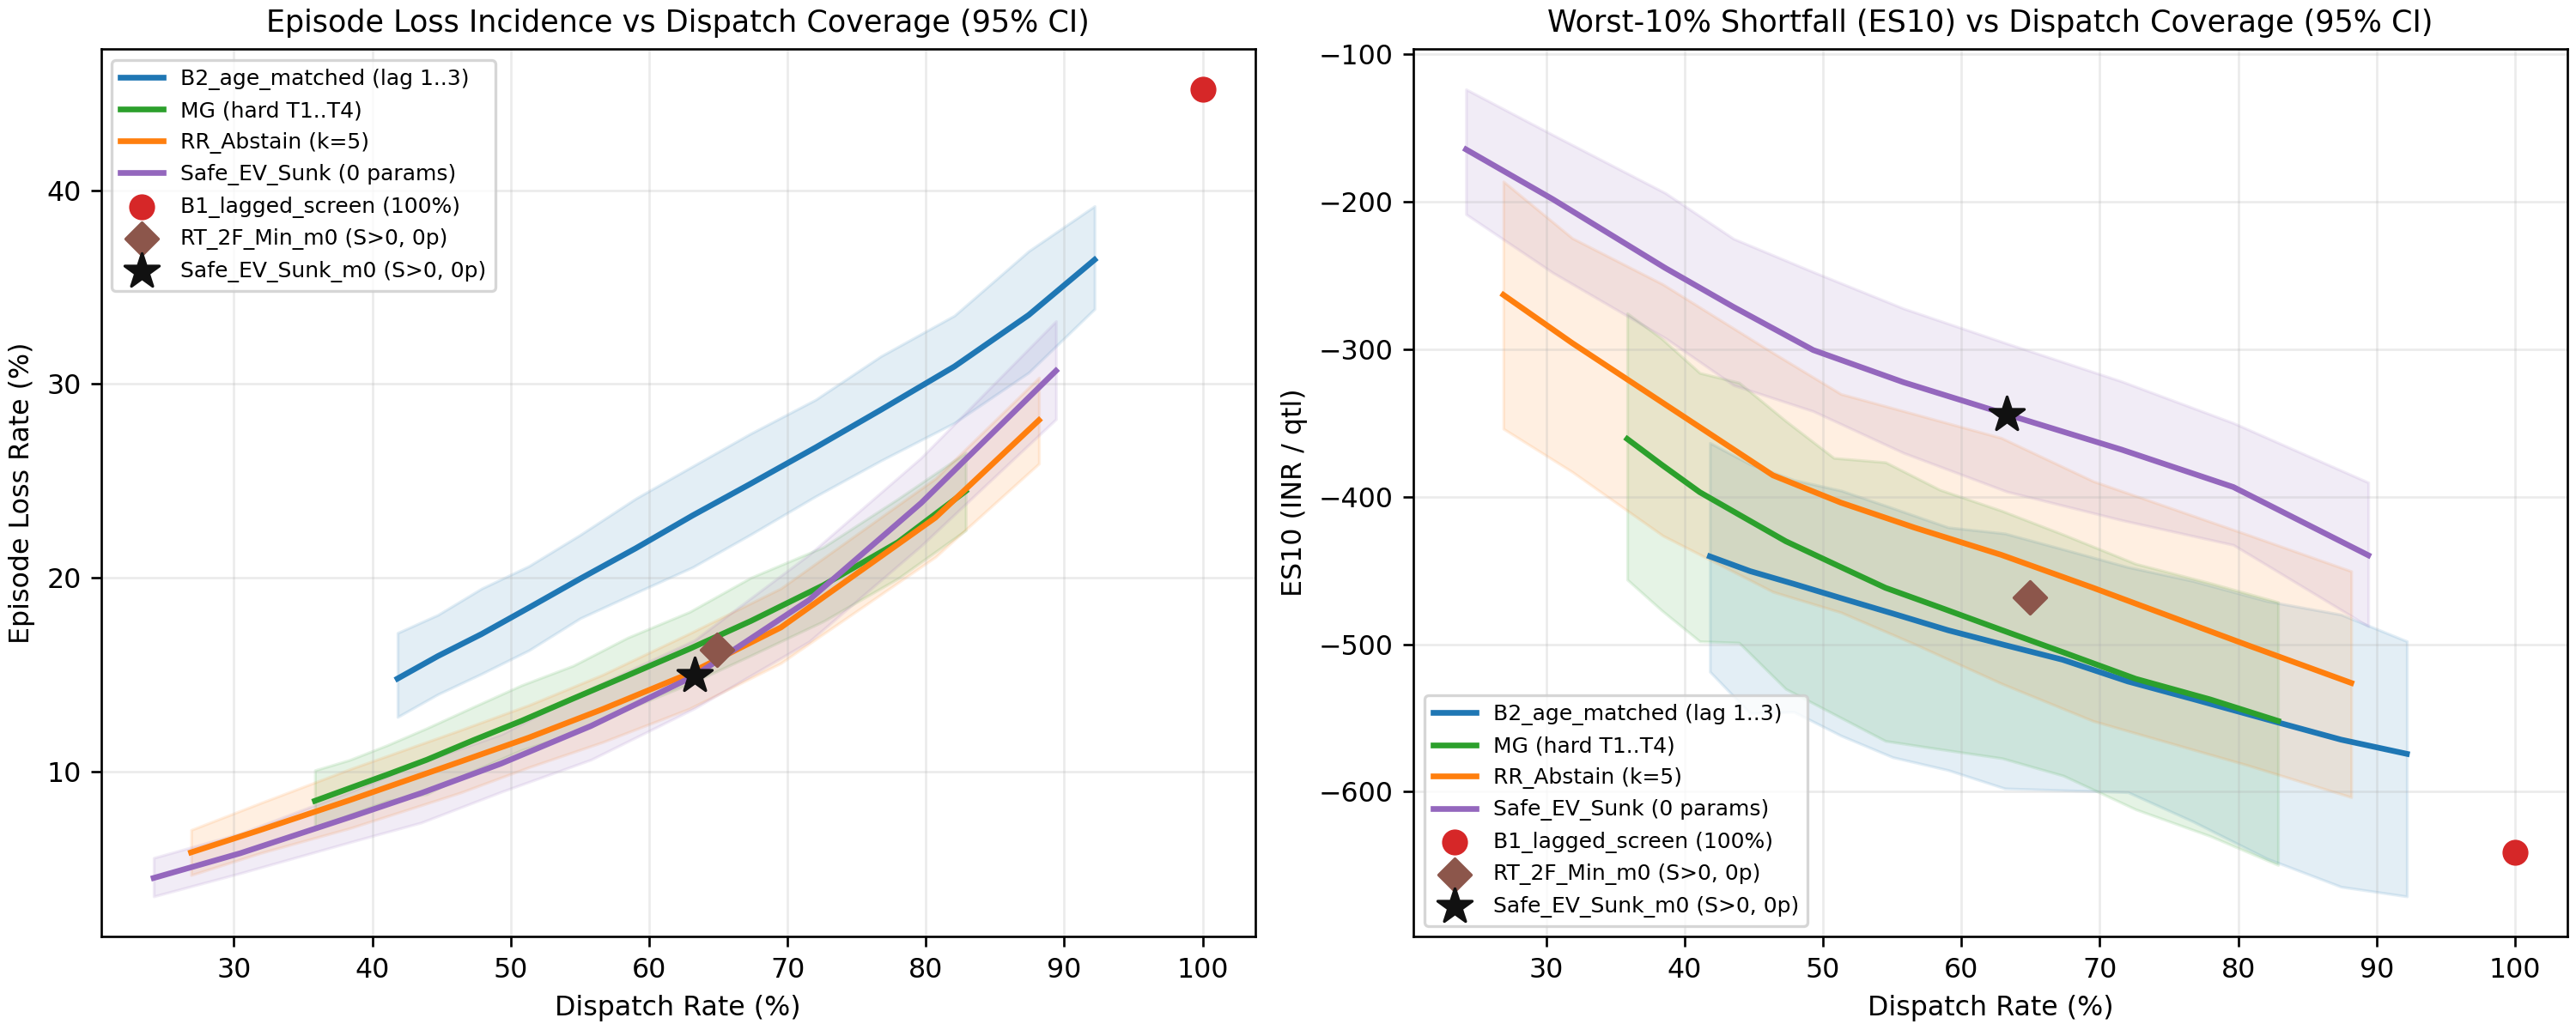
\includegraphics[width=0.96\linewidth]{../figures/rev_fig1_risk_coverage_ci.png}
\caption{Risk-coverage curves with 95\% cluster confidence bands across B2\_age\_matched, hard-gated MG, RR\_Abstain, and zero-parameter Safe\_EV\_Sunk alongside B1 and RT\_2F\_Min}
\end{figure}

\begin{figure}[htbp]
\centering
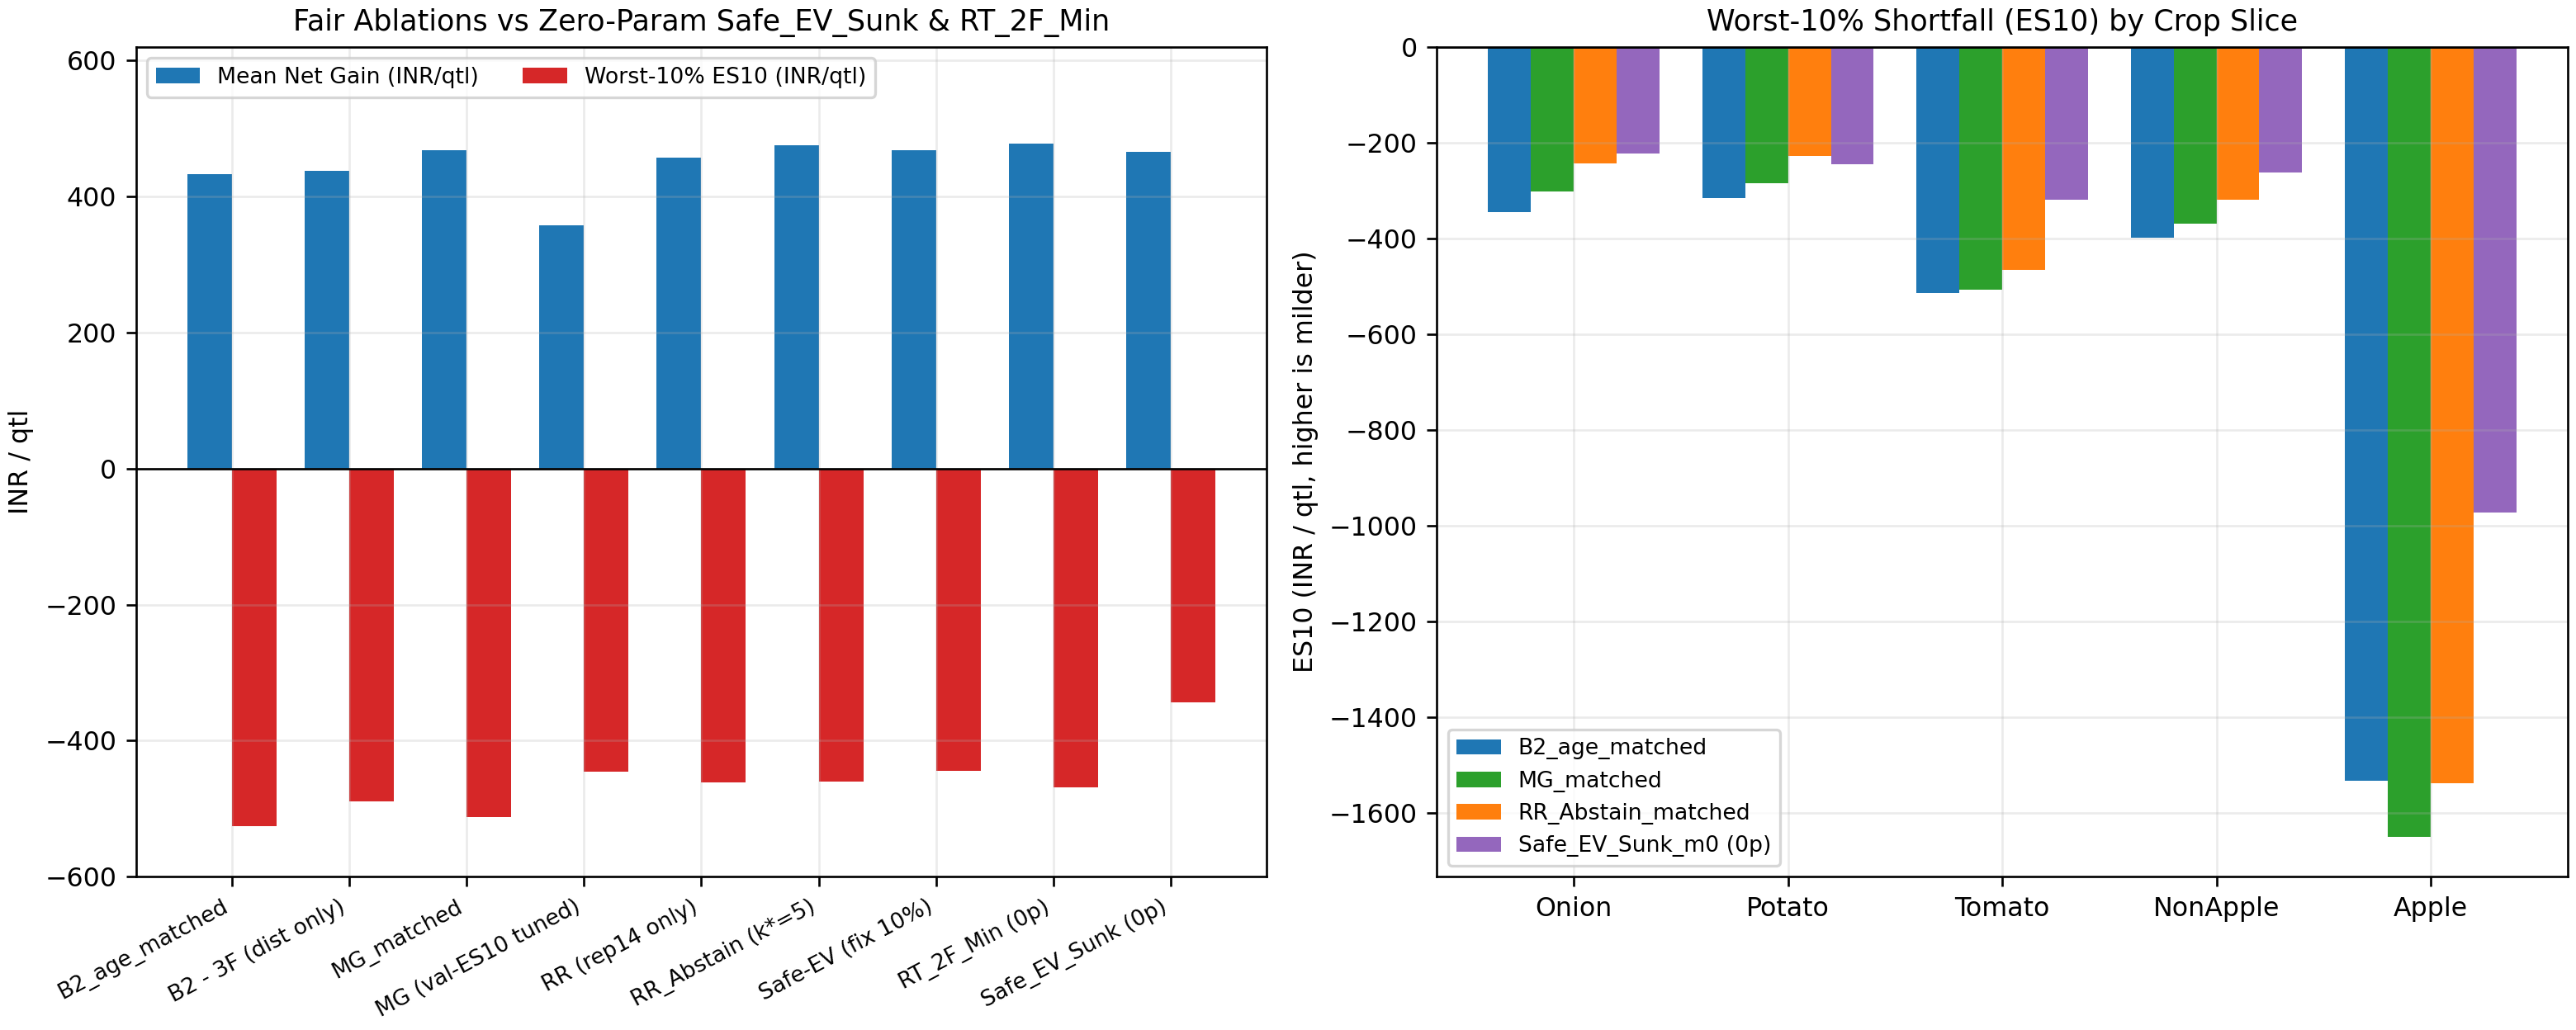
\includegraphics[width=0.96\linewidth]{../figures/rev_fig2_ablations_and_crops.png}
\caption{Fair ablations against Safe\_EV\_Sunk\_m0 and RT\_2F\_Min\_m0 (left) and worst-10\% ES10 comparison across Onion, Potato, Tomato, NonApple, and Apple subsets (right)}
\end{figure}

\subsection{RQ3: Identification Bounds, Subgroup Generalizability, and Stress Audits}

\begin{enumerate}
  \item \textbf{Full Manski and Missing-Quote Regimes (Table 6 \& Figure 3 Right; \texttt{R = 1,000} unadjusted origin-cluster p-values in \texttt{a18\_summary.json}):} Under \texttt{div\_0.0\_spoil\_only} (where code still charges transit spoilage \texttt{-local * spoil < 0}), \texttt{RR\_Abstain\_matched}'s \texttt{ES10} gap over \texttt{B2} falls to statistical noise (\texttt{+Rs.\,9.81}, CI \texttt{[-Rs.\,23.70, +Rs.\,45.94]}, \texttt{p\_2s = 0.603}). Under literal \texttt{exact\_zero\_divert\_payoff\_0}, \texttt{RR} records higher episode loss than \texttt{B2} (\texttt{7.40\%} vs \texttt{6.55\%}, \texttt{p\_2s = 0.032}). \textbf{By contrast, zero-parameter \texttt{Safe\_EV\_Sunk\_m0} retains large tail gains across every non-MAR regime} (\texttt{+Rs.\,173.65 ES10} at \texttt{div\_0.0\_spoil\_only}; \texttt{+Rs.\,169.79 ES10} and \texttt{4.52\%} vs \texttt{6.55\%} losses at \texttt{exact\_zero\_divert\_payoff\_0}, both \texttt{p\_2s = 0.002}). Under the optimistic upper bound where every silent yard actually cleared at \texttt{dest\_lag\_price} (\texttt{open\_yard\_MAR\_lagged\_price}, settling \texttt{no\_comm\_divert\_d0..d2} at day-0 lagged price without wait detention), we disclose explicitly that \textbf{\texttt{B2\_age\_matched} earns \texttt{+Rs.\,102.58/qtl} higher mean} (\texttt{Rs.\,722.66} vs \texttt{Rs.\,620.08}, \texttt{p\_2s = 0.002}), while \texttt{Safe\_EV\_Sunk\_m0} still lowers loss incidence (\texttt{4.78\%} vs \texttt{7.08\%}) and improves \texttt{ES10} by \textbf{\texttt{+Rs.\,190.00/qtl}} (\texttt{-Rs.\,191.91} vs \texttt{-Rs.\,381.91}, \texttt{p\_2s = 0.002}). Restricted solely to realized open \texttt{exact\_d0} auctions (\texttt{n = 30,831} \texttt{Safe\_EV} vs \texttt{30,062} \texttt{B2}), \texttt{Safe\_EV\_Sunk\_m0} halves \texttt{ES10} (\texttt{-Rs.\,307.70} vs \texttt{-Rs.\,623.62}) and nearly matches \texttt{B2} on mean (\texttt{Rs.\,924.65} vs \texttt{Rs.\,930.65}), whereas \texttt{RR} trails \texttt{B2} by \texttt{-Rs.\,94.44}.
\end{enumerate}

\begin{table}[htbp]
\centering
\small
\caption{Missing-quote counterfactual identification bounds from harsh diversion (div = 2.0) to optimistic open-yard MAR settlement.}\label{tab:table6}
\resizebox{\linewidth}{!}{
\begin{tabular}{lllll}
\toprule
Missing-Quote Counterfactual Regime (\texttt{a18\_missing\_regimes.csv}) & \texttt{B2\_age} (Mean / EpL / \texttt{ES10}) & \texttt{RR\_matched} (Mean / EpL / \texttt{ES10}) & \texttt{Safe\_EV\_Sunk\_m0} (Mean / EpL / \texttt{ES10}) & \texttt{RT\_2F\_Min\_m0} (Mean / EpL / \texttt{ES10}) \\
\midrule
\texttt{div\_2.0\_disc\_0.10} \textit{(Harsh diversion)} & \texttt{Rs.\,419.73} / \texttt{26.72\%} / \texttt{-Rs.\,593.52} & \texttt{Rs.\,469.43} / \texttt{17.23\%} / \texttt{-Rs.\,506.17} & \texttt{Rs.\,458.92} / \textbf{\texttt{14.93\%}} / \textbf{\texttt{-Rs.\,400.99}} & \textbf{\texttt{Rs.\,472.57}} / \texttt{16.26\%} / \texttt{-Rs.\,513.26} \\
\texttt{div\_1.5\_disc\_0.10\_base} \textit{(Baseline)} & \texttt{Rs.\,433.56} / \texttt{26.72\%} / \texttt{-Rs.\,525.25} & \texttt{Rs.\,475.36} / \texttt{17.23\%} / \texttt{-Rs.\,460.72} & \texttt{Rs.\,465.59} / \textbf{\texttt{14.93\%}} / \textbf{\texttt{-Rs.\,344.09}} & \textbf{\texttt{Rs.\,478.38}} / \texttt{16.26\%} / \texttt{-Rs.\,468.32} \\
\texttt{div\_0.0\_spoil\_only} \textit{(Still \texttt{-loc*sp})} & \texttt{Rs.\,475.80} / \texttt{26.67\%} / \texttt{-Rs.\,359.17} & \texttt{Rs.\,493.37} / \texttt{17.21\%} / \texttt{-Rs.\,349.35} \textit{(NS)} & \texttt{Rs.\,485.92} / \textbf{\texttt{14.92\%}} / \textbf{\texttt{-Rs.\,185.52}} & \textbf{\texttt{Rs.\,496.01}} / \texttt{16.25\%} / \texttt{-Rs.\,352.72} \\
\texttt{exact\_zero\_divert\_payoff\_0} \textit{(Literal \texttt{Rs.\,0})} & \texttt{Rs.\,477.14} / \texttt{6.55\%} / \texttt{-Rs.\,349.01} & \texttt{Rs.\,494.14} / \texttt{7.40\%} / \texttt{-Rs.\,343.03} \textit{(NS)} & \texttt{Rs.\,486.50} / \textbf{\texttt{4.52\%}} / \textbf{\texttt{-Rs.\,179.22}} & \textbf{\texttt{Rs.\,496.73}} / \texttt{6.58\%} / \texttt{-Rs.\,346.08} \\
\texttt{open\_yard\_MAR\_lagged\_price} \textit{(MAR open)} & \textbf{\texttt{Rs.\,722.66}} / \texttt{7.08\%} / \texttt{-Rs.\,381.91} & \texttt{Rs.\,641.41} / \texttt{7.71\%} / \texttt{-Rs.\,359.16} & \texttt{Rs.\,620.08} / \textbf{\texttt{4.78\%}} / \textbf{\texttt{-Rs.\,191.91}} & \texttt{Rs.\,630.70} / \texttt{6.87\%} / \texttt{-Rs.\,361.51} \\
\texttt{realized\_exact\_d0\_dispatched\_only} \textit{(Open)} & \textbf{\texttt{Rs.\,930.65}} / \texttt{12.10\%} / \texttt{-Rs.\,623.62} & \texttt{Rs.\,836.21} / \texttt{12.33\%} / \texttt{-Rs.\,563.99} & \texttt{Rs.\,924.65} / \textbf{\texttt{8.31\%}} / \textbf{\texttt{-Rs.\,307.70}} & \texttt{Rs.\,900.16} / \texttt{11.74\%} / \texttt{-Rs.\,608.10} \\
\texttt{het\_adversarial\_lowrep\_ok\_highrep\_harsh} & \texttt{Rs.\,435.33} / \texttt{26.69\%} / \texttt{-Rs.\,569.44} & \texttt{Rs.\,470.54} / \texttt{17.23\%} / \texttt{-Rs.\,503.84} & \texttt{Rs.\,463.12} / \textbf{\texttt{14.93\%}} / \textbf{\texttt{-Rs.\,385.31}} & \textbf{\texttt{Rs.\,474.43}} / \texttt{16.26\%} / \texttt{-Rs.\,508.53} \\
\bottomrule
\end{tabular}}
\end{table}

\begin{enumerate}
  \setcounter{enumi}{1}
  \item \textbf{All 6 Individual States and All 5 Crop Slices (\texttt{a18\_crop\_and\_state\_splits.csv}):} Unlike \texttt{RR\_Abstain\_matched} (whose \texttt{ES10} CIs cross zero in Maharashtra \texttt{[-Rs.\,68.87, +Rs.\,68.33]} and HP \texttt{[-Rs.\,19.98, +Rs.\,169.84]}), \textbf{\texttt{Safe\_EV\_Sunk\_m0} yields strictly positive 95\% \texttt{ES10} CIs in all six states}: Gujarat \texttt{[+Rs.\,138.05, +Rs.\,369.11]}, HP \texttt{[+Rs.\,59.18, +Rs.\,637.28]}, Karnataka \texttt{[+Rs.\,58.23, +Rs.\,184.08]}, MP \texttt{[+Rs.\,139.94, +Rs.\,303.97]}, Maharashtra \texttt{[+Rs.\,48.71, +Rs.\,303.07]}, and UP \texttt{[+Rs.\,48.00, +Rs.\,139.86]}, and across \textbf{all five crop slices} (\texttt{NonApple} \texttt{N = 52,207}: \texttt{+Rs.\,135.58} CI \texttt{[+Rs.\,108.37, +Rs.\,165.94]}; Onion \texttt{+Rs.\,123.49}; Potato \texttt{+Rs.\,72.31}; Tomato \texttt{+Rs.\,195.65}; generic Apple \texttt{N = 6,469}: \texttt{+Rs.\,561.37} CI \texttt{[+Rs.\,172.22, +Rs.\,1,216.91]}). On \textbf{mean net gain} vs \texttt{B2\_age\_matched}, \texttt{Safe\_EV\_Sunk\_m0}'s 95\% CIs cross zero in Gujarat (\texttt{Rs.\,344.63} vs \texttt{Rs.\,346.29}, CI \texttt{[-Rs.\,49.29, +Rs.\,36.56]}), Maharashtra (\texttt{CI [-Rs.\,5.58, +Rs.\,36.32]}), UP (\texttt{CI [-Rs.\,3.18, +Rs.\,27.00]}), Tomato (\texttt{Rs.\,461.42} vs \texttt{Rs.\,462.27}, CI \texttt{[-Rs.\,34.58, +Rs.\,28.50]}), and Apple (\texttt{CI [-Rs.\,24.81, +Rs.\,245.04]}) due to conservative volatility filtering, whereas zero-parameter \textbf{\texttt{RT\_2F\_Min\_m0}} beats \texttt{B2}'s point mean in all six states and all five crop slices (\texttt{Tomato Rs.\,504.35}).
  \item \textbf{18-Scenario Frozen and Re-Scored Tornado (\texttt{a18\_tornado.csv}):} Across all 18 freight, commission, hill-factor, spoilage, and detention regimes (\texttt{NITI Rs.\,0.258/km} floor, LCV \texttt{Rs.\,0.75/km}, steep \texttt{Rs.\,1.20/km}, HP \texttt{1.00--1.75}, \textit{arhtiya} \texttt{2--6\%}, \texttt{buyer\_paid\_0\%}, \texttt{spoil 0.5--2x}, \texttt{detention 0--100}, \texttt{joint\_optimistic}, \texttt{joint\_harsh}, \texttt{outside\_origin\_lag}) under both frozen and re-scored policies (\texttt{36} cells), \textbf{\texttt{Safe\_EV\_Sunk\_m0} outperforms \texttt{B2\_age\_matched} in 36 of 36 cells on both Mean (\texttt{+Rs.\,13.31} to \texttt{+Rs.\,61.11}) and \texttt{ES10} (\texttt{+Rs.\,144.94} to \texttt{+Rs.\,329.37})}, with zero sign reversals.
  \item \textbf{Structural Integrity and Unconditional Origin Panel (\texttt{a18\_settlement\_and\_robustness.csv}):} \texttt{Safe\_EV\_Sunk\_m0} improves over \texttt{B2\_age\_matched} on \texttt{exact\_geocode\_corridors\_only} (\texttt{N = 40,690} episodes retaining exact-geocoded corridors after excluding centroid endpoints: \texttt{ES10 -Rs.\,364.46} vs \texttt{-Rs.\,556.97}, ep\_loss \texttt{13.33\%} vs \texttt{24.38\%}; all-5 exact episodes \texttt{N = 18,189} behave consistently), \texttt{non\_conflicting\_dup\_episodes\_only} (\texttt{N = 56,857}: \texttt{-Rs.\,343.85} vs \texttt{-Rs.\,520.66}), \texttt{origin\_lag\_age\_1\_3\_only} (\texttt{N = 56,648}: \texttt{-Rs.\,339.91} vs \texttt{-Rs.\,522.40}), \texttt{hindsight\_3d} (\texttt{-Rs.\,281.99} vs \texttt{-Rs.\,591.16}), and the \textbf{\texttt{N = 88,014} unconditional origin panel} restoring all \texttt{29,338} unreported day-$t$ origin episodes (\texttt{Safe\_EV\_Sunk\_m0}: Mean \texttt{Rs.\,483.03} vs \texttt{Rs.\,445.37}, EpLoss \texttt{15.22\%} vs \texttt{28.10\%}, \textbf{\texttt{ES10 -Rs.\,335.04} vs \texttt{-Rs.\,515.93}}; \texttt{RT\_2F\_Min\_m0}: Mean \textbf{\texttt{Rs.\,493.15}}).
  \item \textbf{HP Graded Apples (\texttt{a18\_hp\_apple.csv} --- Stress Check):} Across \texttt{N = 2,802} lagged HP graded-apple episodes (\texttt{2025-11..2026-08}), zero-parameter \textbf{\texttt{Safe\_EV\_Sunk\_m0} (\texttt{67.45\%} disp)} achieves Mean \textbf{\texttt{Rs.\,1,354.85}} (vs \texttt{B2} \texttt{Rs.\,1,199.31}, \texttt{MG\_matched} \texttt{Rs.\,1,028.05}, \texttt{RR} \texttt{Rs.\,1,318.60}) and narrows \texttt{ES10} to \textbf{\texttt{-Rs.\,1,454.86}} (\texttt{+Rs.\,937.26} over \texttt{B2} \texttt{-Rs.\,2,392.12}, \texttt{+Rs.\,498.34} over \texttt{MG\_matched} \texttt{-Rs.\,1,953.20}, \texttt{+Rs.\,710.87} over \texttt{RR} \texttt{-Rs.\,2,165.73}; \texttt{Safe\_EV\_Phys\_m0} attains \texttt{-Rs.\,1,376.71}), extending into June--August 2026 (\texttt{Rs.\,2,010.20} mean, \texttt{-Rs.\,2,479.28} vs \texttt{B2 -Rs.\,4,071.95}). Still, \textbf{\texttt{41.38\%}} of dispatched HP apple trips lose money (\texttt{-Rs.\,1,454.86} tail), underscoring that high-variance graded apples require live buyer confirmation prior to truck loading.
\end{enumerate}

\begin{figure}[htbp]
\centering
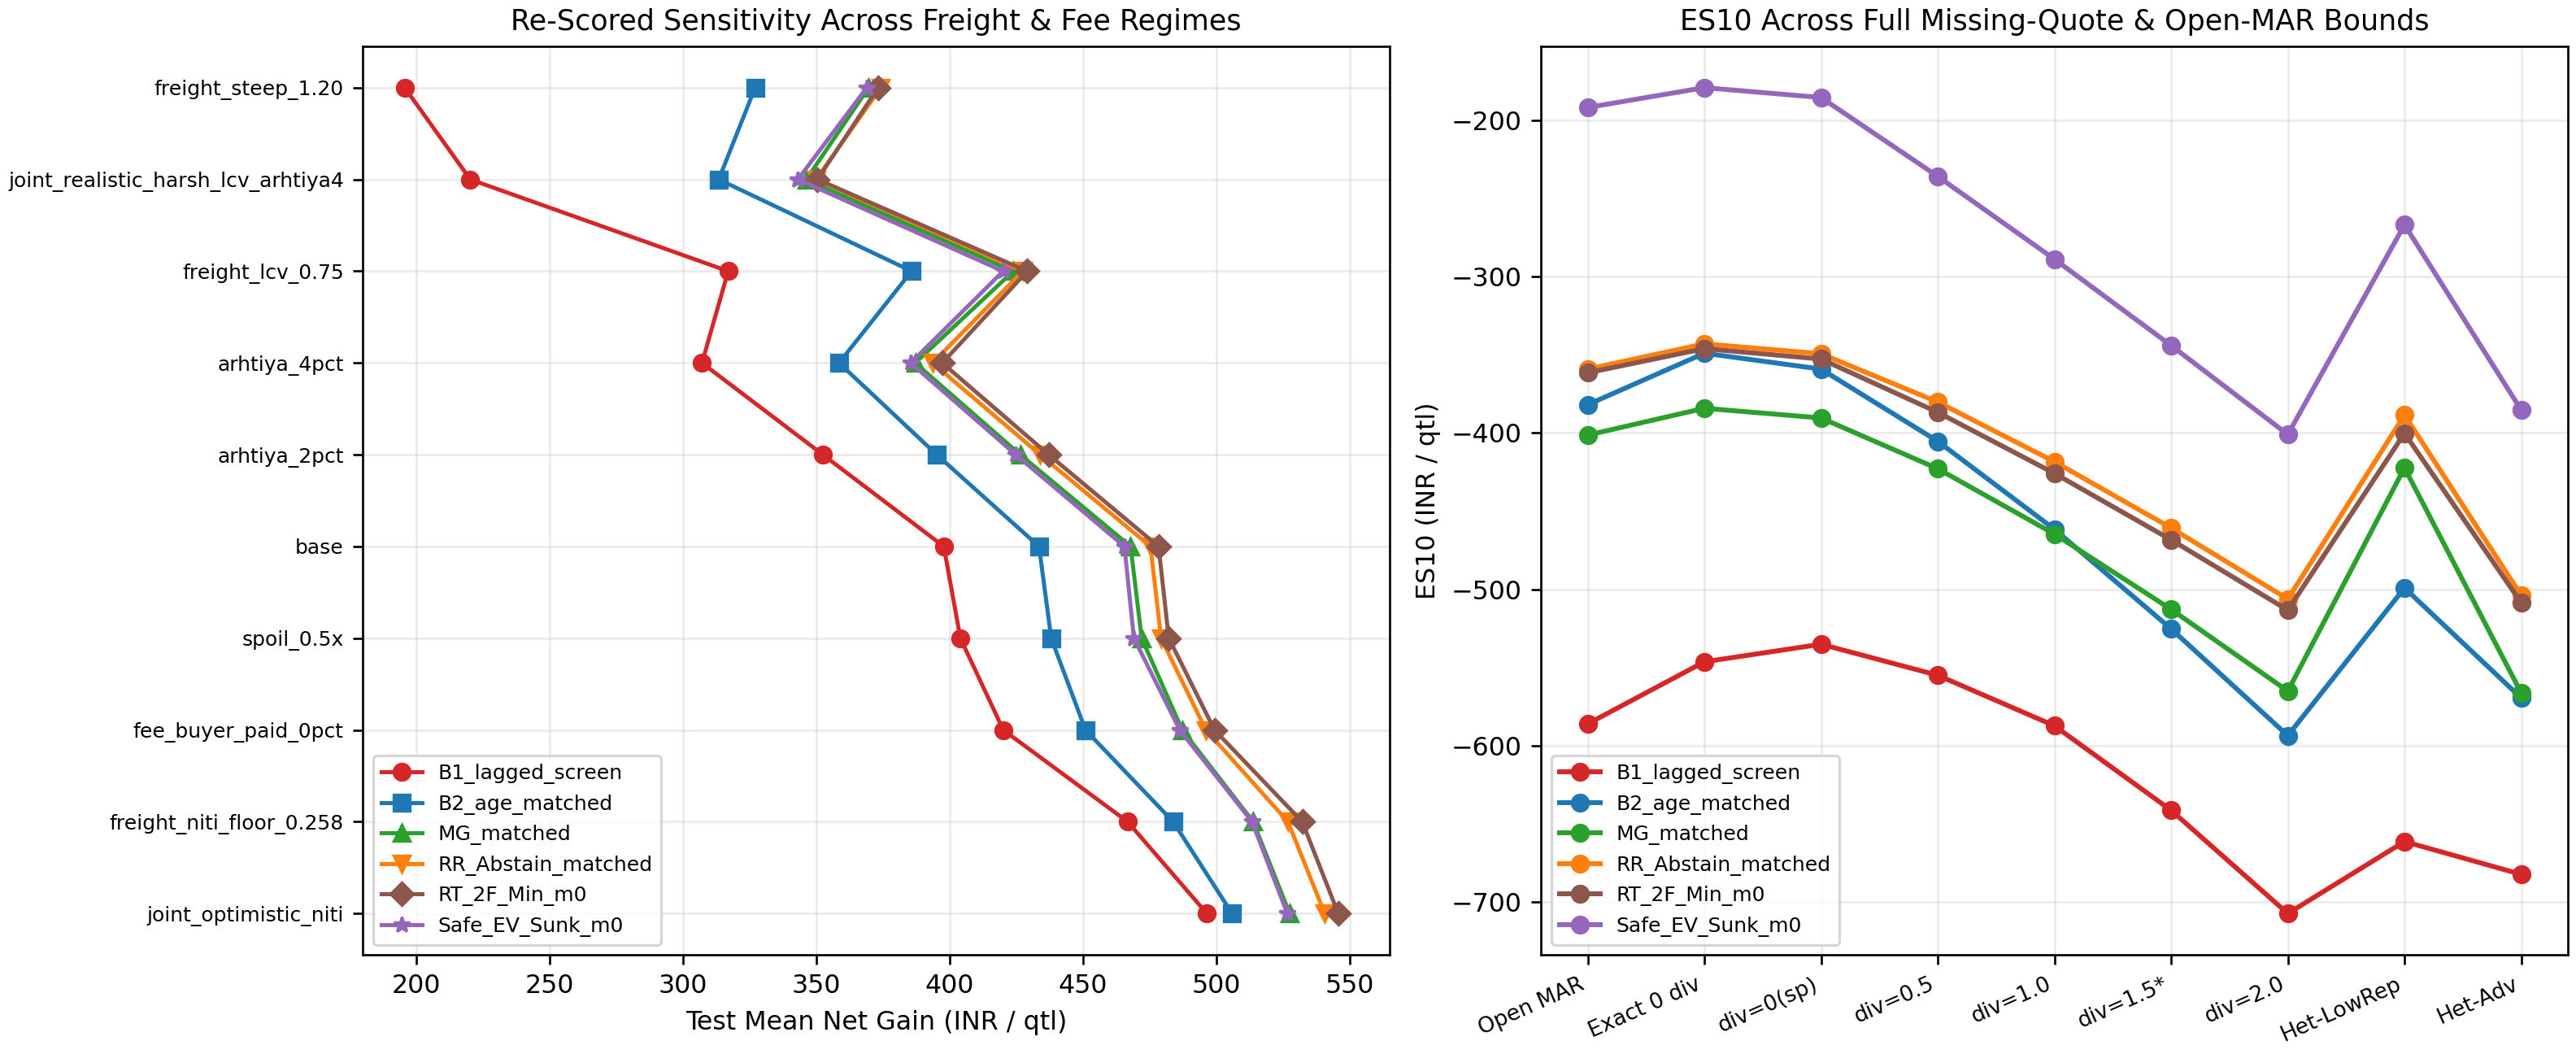
\includegraphics[width=0.96\linewidth]{../figures/rev_fig3_sensitivity_tornado_and_missing.png}
\caption{Re-scored parameter sensitivity across 10 representative freight and commission regimes from the 18-scenario tornado (a18\_tornado.csv, left) and ES10 across complete missing-quote and Open-MAR identification bounds (right)}
\end{figure}

\begin{figure}[htbp]
\centering
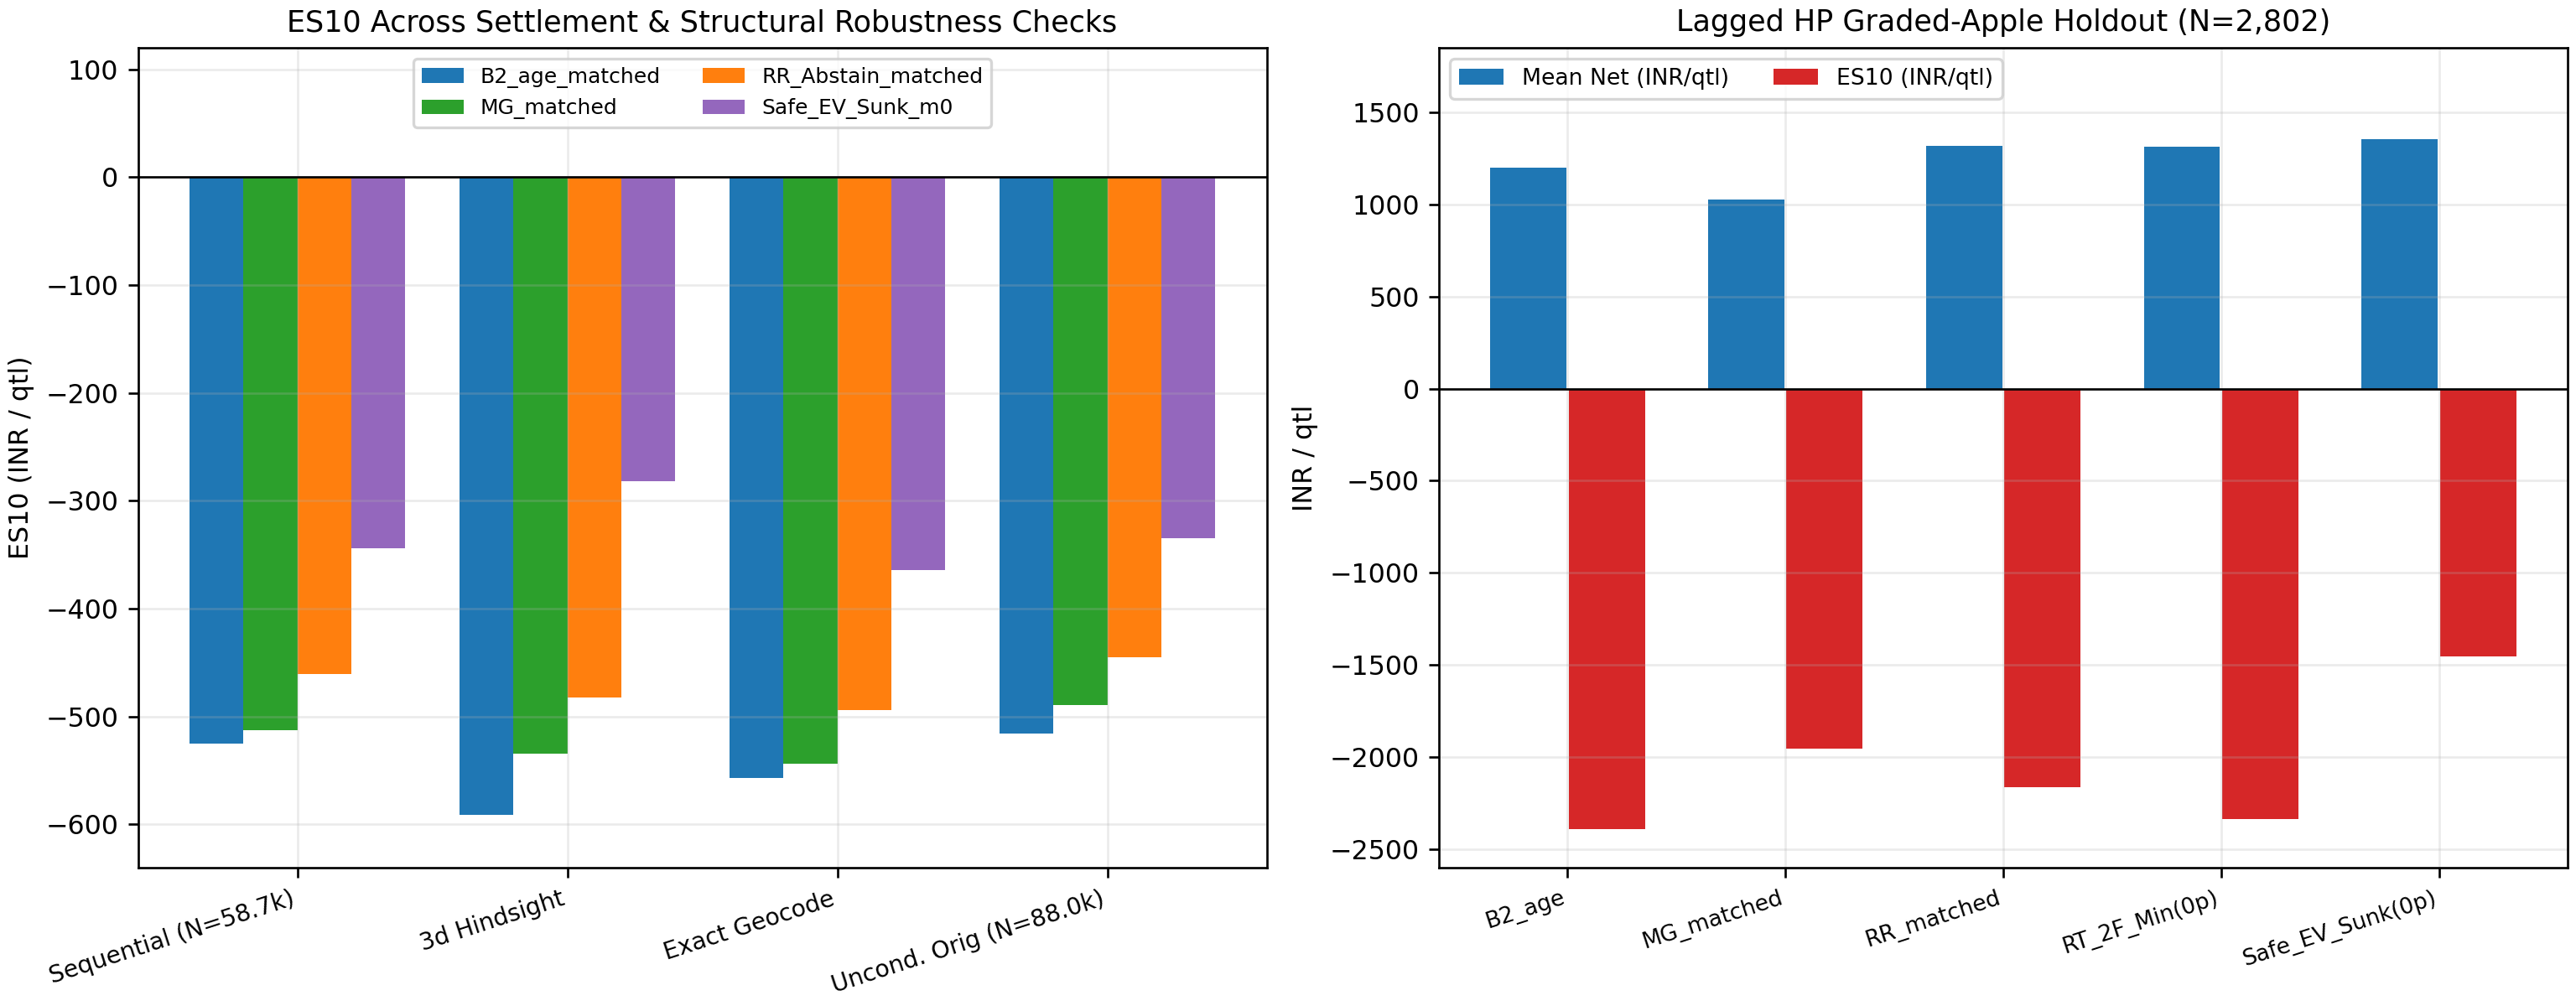
\includegraphics[width=0.96\linewidth]{../figures/rev_fig4_settlement_and_hp_apple.png}
\caption{ES10 across sequential, hindsight, exact-geocode, and N=88,014 unconditional origin panels (left) and lagged HP graded-apple holdout performance (right)}
\end{figure}

\subsection{\texttt{Revision v6} Robustness: Fresh \texttt{2024}-Only \texttt{171}-Market Rebuild, Realized ERA5 Settlement, Exact Break-Even, and \texttt{1w}/\texttt{4w} Block Checks}

To address four deeper referee concerns directly on committed files (\texttt{revision/eval\_v6.py}, \texttt{v6\_upgrades.csv}, \texttt{v6\_breakeven.csv}, \texttt{v6\_bootstrap\_5000.csv}), Table 7 reports:

\begin{enumerate}
  \item \textbf{Fresh End-to-End \texttt{2024}-Only \texttt{171}-Market Rebuild (\texttt{N = 57,634} test episodes, \texttt{195,421} shortlisted rows, \texttt{166} clusters):} Selecting eligible markets exclusively from \texttt{2024} records (\texttt{>= 80} days, \texttt{<= 30}/state $\to$ \texttt{GJ 30, HP 23, KA 28, MP 30, MH 30, UP 30}), rebuilding Top-5 lagged shortlists from scratch on those \texttt{171} raw markets (avoiding any post-hoc Top-5 truncation), and re-calibrating \texttt{B2} and matched comparators strictly on \texttt{val\_171} (\texttt{tune\_threshold\_on\_val} keeps \texttt{th\_b2 = Rs.\,200.00}) eliminates any post-2024 market-inclusion lookahead. Results remain virtually unchanged: \texttt{Safe\_EV\_Sunk\_m0} improves \texttt{ES10} by \texttt{+Rs.\,179.24/qtl} under \texttt{20$^\circ$C} (\texttt{p\_holm\_2s = 0.0024}; \texttt{H\_V6\_4} \texttt{0.0024--0.0032}; \texttt{H\_V6\_6} Mean \texttt{+Rs.\,33.12}, \texttt{p\_holm\_2s = 0.0032} origin / \texttt{0.0408} B2-dest) and by \texttt{+Rs.\,187.80/qtl} under realized ERA5 (\texttt{Safe\_EV\_Phys\_m0} \texttt{+Rs.\,199.07/qtl}, \texttt{p\_holm\_2s = 0.0024}; \texttt{H\_V6\_6} Mean \texttt{+Rs.\,34.55}, \texttt{p\_holm\_2s = 0.0024} origin / \texttt{0.0320} B2-dest).
  \item \textbf{Realized ERA5 Destination Arrival-Day Weather Settlement (\texttt{100.0\%} coordinate-day coverage across \texttt{d0..d2}, zero weather in decisions):} Scoring the identical weather-free \texttt{<= t - 1} policies against realized destination arrival-day heat, humidity, and heavy rain (\texttt{>= 35 mm} price-to-min compression and \texttt{+0.02} rot penalty) lowers raw payoffs across every rule by \texttt{Rs.\,13--19/qtl} while \textbf{widening the zero-parameter advantage}: on \texttt{178} markets, \texttt{Safe\_EV\_Sunk\_m0} gains \textbf{\texttt{+Rs.\,190.43/qtl} \texttt{ES10}} (\texttt{-Rs.\,364.28} vs \texttt{-Rs.\,554.71}, \texttt{p\_holm\_2s = 0.0024}), \texttt{Safe\_EV\_Phys\_m0} gains \textbf{\texttt{+Rs.\,201.55/qtl} \texttt{ES10}} (\texttt{-Rs.\,353.16}), and \texttt{RT\_2F\_Min\_m0} leads mean at \texttt{Rs.\,464.36/qtl} (\texttt{+Rs.\,45.35}, \texttt{p\_holm\_2s = 0.0024}). Under realized ERA5 Open-Yard MAR (which replaces \texttt{no\_comm\_divert\_d0..d2} with day-0 lagged sales at realized \texttt{d0} weather and zero detention), \texttt{B2} retains \texttt{+Rs.\,100.57/qtl} higher mean (\texttt{Rs.\,707.04} vs \texttt{Rs.\,606.48} rounded), while \texttt{Safe\_EV\_Sunk\_m0} narrows \texttt{ES10} by \texttt{+Rs.\,196.38/qtl} (\texttt{-Rs.\,205.73} vs \texttt{-Rs.\,402.11}).
  \item \textbf{Algebraically Exact Silent-Market Break-Even Thresholds (\texttt{16} rows, \texttt{verification\_resid = 0.0}):} Because \texttt{Safe\_EV\_Sunk\_m0} encounters silent arrival yards (\texttt{no\_comm\_divert}) on \texttt{10.41\%} of episodes versus \texttt{20.16\%} for \texttt{B2\_age\_matched}, we compute three distinct homogeneous break-even counterfactuals where mean payoffs equalize: (a) \textbf{Uniform shift above each policy's closed-yard turn-back:} \texttt{B2} overtakes \texttt{Safe\_EV\_Sunk\_m0} on mean only if silent trips average \textbf{\texttt{+Rs.\,328.37/qtl} above closed-yard turn-back} (\texttt{+Rs.\,343.84} under ERA5; \texttt{+Rs.\,348.61} on rebuilt \texttt{171}-mkt \texttt{20$^\circ$C}; \texttt{+Rs.\,363.74} on \texttt{171}-mkt ERA5); (b) \textbf{Separate flat constant-payoff counterfactual} setting \textit{both} policies' silent trips to an identical net profit above local (removing \texttt{Safe\_EV}'s shorter-corridor lower turn-back loss): \textbf{\texttt{+Rs.\,95.97/qtl}} (\texttt{+Rs.\,97.25} ERA5; \texttt{+Rs.\,117.97} \texttt{171}-mkt \texttt{20$^\circ$C}; \texttt{+Rs.\,119.16} \texttt{171}-mkt ERA5); and (c) \textbf{Homogeneous Open-MAR mixture share $\theta^*$:} \textbf{\texttt{23.79\%}} (\texttt{25.01\%} ERA5; \texttt{25.45\%} \texttt{171}-mkt \texttt{20$^\circ$C}; \texttt{26.65\%} \texttt{171}-mkt ERA5) of silent yards clearing at full lagged prices. For \texttt{RT\_2F\_Min\_m0} vs \texttt{B2}, uniform shift break-even is \textbf{\texttt{+Rs.\,427.54/qtl}} (flat constant payoff \texttt{+Rs.\,186.84/qtl}; \texttt{32.77\%} MAR share; \texttt{+Rs.\,438.73} / \texttt{34.45\%} on \texttt{171}-mkt ERA5).
  \item \textbf{Calendar Block-Length Sensitivity (\texttt{R = 5,000}):} Across \texttt{1}-week (\texttt{45} blocks), \texttt{2}-week (\texttt{23} blocks), and \texttt{4}-week (\texttt{12} blocks---noted as a small-cluster temporal sensitivity check) resamplings, every contrast \texttt{H\_V6\_1..H\_V6\_6} remains statistically significant (\texttt{p\_holm\_2s = 0.0024} for all tail/loss/\texttt{RT}-mean tests; \texttt{Safe\_EV} mean \texttt{p\_holm\_2s = 0.0024} [\texttt{1w}], \texttt{0.0028} [\texttt{2w}], \texttt{0.0040} [\texttt{4w}]).
\end{enumerate}

\begin{table}[htbp]
\centering
\small
\caption{Revision v6 robustness panels comparing full 178-market and freshly rebuilt strict 2024-only 171-market panels under 20$^\circ$C reference and realized ERA5 arrival-day weather, with exact silent-market break-even thresholds.}\label{tab:table7}
\resizebox{\linewidth}{!}{
\begin{tabular}{llllll}
\toprule
Verification Panel (\texttt{v6\_upgrades.csv} \& \texttt{v6\_breakeven.csv}) & \texttt{B2\_age} (Mean / EpL / \texttt{ES10}) & \texttt{Safe\_EV\_Sunk\_m0} (Mean / EpL / \texttt{ES10}) & \texttt{Safe\_EV\_Phys\_m0} (Mean / EpL / \texttt{ES10}) & \texttt{RT\_2F\_Min\_m0} (Mean / EpL / \texttt{ES10}) & \texttt{Safe\_EV} vs \texttt{B2} Break-Even (Shift / Flat / MAR\%) \\
\midrule
\texttt{full\_178\_20C\_closed} (\texttt{N = 58,676}) & \texttt{Rs.\,433.56} / \texttt{26.72\%} / \texttt{-Rs.\,525.25} & \texttt{Rs.\,465.59} / \texttt{14.93\%} / \texttt{-Rs.\,344.09} & \texttt{Rs.\,462.16} / \texttt{13.73\%} / \texttt{-Rs.\,333.57} & \texttt{Rs.\,478.38} / \texttt{16.26\%} / \texttt{-Rs.\,468.32} & \texttt{+Rs.\,328.37} / \texttt{+Rs.\,95.97} / \texttt{23.79\%} \\
\texttt{full\_178\_ERA5\_closed} (\texttt{N = 58,676}) & \texttt{Rs.\,419.01} / \texttt{26.99\%} / \texttt{-Rs.\,554.71} & \texttt{Rs.\,452.55} / \texttt{15.20\%} / \texttt{-Rs.\,364.28} & \texttt{Rs.\,449.40} / \texttt{13.99\%} / \texttt{-Rs.\,353.16} & \texttt{Rs.\,464.36} / \texttt{16.56\%} / \texttt{-Rs.\,493.63} & \texttt{+Rs.\,343.84} / \texttt{+Rs.\,97.25} / \texttt{25.01\%} \\
\texttt{full\_178\_ERA5\_open\_MAR} (\texttt{N = 58,676}) & \textbf{\texttt{Rs.\,707.04}} / \texttt{7.38\%} / \texttt{-Rs.\,402.11} & \texttt{Rs.\,606.48} / \texttt{5.06\%} / \textbf{\texttt{-Rs.\,205.73}} & \texttt{Rs.\,594.09} / \textbf{\texttt{4.74\%}} / \textbf{\texttt{-Rs.\,198.97}} & \texttt{Rs.\,616.16} / \texttt{7.17\%} / \texttt{-Rs.\,381.64} & \textit{(Upper MAR endpoint)} \\
\texttt{strict2024\_171\_20C\_closed} (\texttt{N = 57,634}) & \texttt{Rs.\,419.62} / \texttt{26.43\%} / \texttt{-Rs.\,524.78} & \texttt{Rs.\,452.74} / \texttt{14.88\%} / \texttt{-Rs.\,345.53} & \texttt{Rs.\,449.52} / \texttt{13.70\%} / \texttt{-Rs.\,334.80} & \texttt{Rs.\,463.98} / \texttt{16.21\%} / \texttt{-Rs.\,464.84} & \texttt{+Rs.\,348.61} / \texttt{+Rs.\,117.97} / \texttt{25.45\%} \\
\texttt{strict2024\_171\_ERA5\_closed} (\texttt{N = 57,634}) & \texttt{Rs.\,405.73} / \texttt{26.69\%} / \texttt{-Rs.\,552.91} & \texttt{Rs.\,440.28} / \texttt{15.12\%} / \texttt{-Rs.\,365.11} & \texttt{Rs.\,437.31} / \texttt{13.94\%} / \texttt{-Rs.\,353.85} & \texttt{Rs.\,450.56} / \texttt{16.50\%} / \texttt{-Rs.\,489.02} & \texttt{+Rs.\,363.74} / \texttt{+Rs.\,119.16} / \texttt{26.65\%} \\
\texttt{strict2024\_171\_ERA5\_open\_MAR} (\texttt{N = 57,634}) & \textbf{\texttt{Rs.\,683.27}} / \texttt{7.37\%} / \texttt{-Rs.\,402.35} & \texttt{Rs.\,588.17} / \texttt{5.03\%} / \textbf{\texttt{-Rs.\,206.82}} & \texttt{Rs.\,576.35} / \textbf{\texttt{4.72\%}} / \textbf{\texttt{-Rs.\,200.08}} & \texttt{Rs.\,597.97} / \texttt{7.14\%} / \texttt{-Rs.\,376.45} & \textit{(Upper MAR endpoint)} \\
\bottomrule
\end{tabular}}
\end{table}

\section{Related Work and Surviving Applied Contribution}

Five research streams frame our audit and design choices:

\begin{enumerate}
  \item \textbf{Spatial Arbitrage, Market Power, and Agricultural Information Services:} Parity-bound models show that gross spreads below transfer costs yield zero arbitrage \cite{baulch1997transfer}, and empirical studies of Indian wholesale integration document persistent spatial wedges driven by transport frictions, market density, and local intermediary power \cite{sekhar2012agricultural,chatterjee2016six,negi2018farmers,mahajan2021covid,chatterjee2023market}. While mobile price discovery reduced fish waste in Kerala \cite{jensen2007digital} and raised soybean prices near hubs \cite{goyal2010information}, randomized SMS and market-information trials show muted or heterogeneous gains when bargaining power, credit ties, or execution frictions bind \cite{fafchamps2012sms,courtois2015farmer,mitra2018asymmetric}, whereas unified e-auction platforms raise realized prices when transaction execution is reliable \cite{levi2020impact,levi2025improving}.
  \item \textbf{Agricultural Price Forecasting and Market Intelligence Systems:} Applied computing systems predict wholesale mandi prices via time-series, collaborative filtering, or deep learning \cite{madaan2019price,ma2019price,guo2020mandi}, study farmer-facing market intelligence workflows \cite{ziegler2019fresh,ladhar2023ai}, or reconstruct missing portal rows using regional factor models \cite{deka2026missing}. Those studies optimize price-prediction RMSE or imputation error rather than evaluating sequential non-reporting arrival execution and worst-decile dispatch shortfall under strict \texttt{<= t - 1} timing.
  \item \textbf{Decision-Focused Learning and Selective Abstention:} Decision-focused learning and smart predict-then-optimize frameworks align scoring directly with downstream operational loss \cite{ban2019bigdata,elmachtoub2022smart,mandi2024dfl}, while reject-option and selective-prediction theory formalizes abstention under asymmetric error costs \cite{chow1970optimum,el_yaniv2010selective,geifman2017selective,franc2023optimal}. Our contribution demonstrates empirically that in thin agricultural portals, simple zero-parameter expected-value ratios using weekday reporting reliability and historical volatility outperform both hard activity thresholds and grid-tuned abstention penalties.
  \item \textbf{Missing-Data Mechanisms, Partial Identification, and Tail Risk:} Rubin's missing-data taxonomy \cite{rubin1976inference}, Manski's nonparametric bounds \cite{manski1990bounds,horowitz2000nonparametric}, selective-label evaluation \cite{lakkaraju2017selective}, and minimax policy learning under unobserved confounding \cite{kallus2021minimax} motivate bracketing unobserved blank arrival rows rather than treating missingness as purely closed or purely open. Tail risk is measured via coherent expected shortfall \cite{rockafellar2000cvar}.
  \item \textbf{Conformal Risk Control and Non-Exchangeable Inference:} Distribution-free conformal prediction, risk control, and conformal decision theory \cite{angelopoulos2023conformal,barber2023beyond,jin2023selection,angelopoulos2024conformal,lekeufack2024conformal} offer finite-sample guarantees under exchangeability or bounded shift, but fail to hold out of the box under action-dependent selective arrival denominators and correlated commodity regimes---explaining why we claim zero conformal guarantees and evaluate via two-way cluster bootstraps with finite-sample Holm corrections \cite{phipson2010permutation,holm1979simple}.
\end{enumerate}

\textbf{Minimal Surviving Applied Contribution:} Claiming no new mathematical theorem or neural architecture, this study establishes in a strictly \texttt{<= t - 1}, sequentially settled retrospective audit (\texttt{N = 58,676}, corroborated on a fresh \texttt{N = 57,634} \texttt{2024}-only market rebuild, realized ERA5 destination arrival-weather settlement, and \texttt{N = 88,014} unconditional origins) that \textbf{replacing black-box trees, hard activity cutoffs, and tuned penalties with zero-hyperparameter expected-value ratios---\texttt{Safe\_EV\_Sunk\_m0} ($p_{\text{dow}} G_{\text{1SD}} > F$), settlement-matched \texttt{Safe\_EV\_Phys\_m0} (\texttt{1.5F}), and Class-8 \texttt{RT\_2F\_Min\_m0} ($p_{\min} G > 2F$)---eliminates tuning parameters while improving worst-10\% \texttt{ES10} over equal-age road dispatch (\texttt{B2\_age\_matched}) by \texttt{+Rs.\,179.24} to \texttt{+Rs.\,201.55/qtl} across the four closed-yard panels (\texttt{p\_holm\_2s = 0.0024} at \texttt{R = 5,000}), with positive 95\% \texttt{ES10} CIs vs \texttt{B2} in every state and crop}. Against tuned \texttt{RR\_Abstain\_matched}, validation-matched \texttt{Safe\_EV\_Sunk\_matched} improves \texttt{ES10} by \texttt{+Rs.\,94.31/qtl} (\texttt{p\_holm\_2s = 0.0024--0.0040}, while threshold-free \texttt{Safe\_EV\_Sunk\_m0} gains \texttt{+Rs.\,116.63/qtl} overall at lower \texttt{63.27\%} vs \texttt{69.02\%} coverage, trails \texttt{RR} by \texttt{-Rs.\,9.77/qtl} on aggregate mean, and trails \texttt{RR} by \texttt{-Rs.\,16.60/qtl} on Potato \texttt{ES10}: \texttt{-Rs.\,243.97} vs \texttt{-Rs.\,227.37}).

\section{Explicit Limitations and Non-Claims}

Eight explicit boundaries govern interpretation and deployment:

\begin{enumerate}
  \item \textbf{Modeled Payoffs $\ne$ Farmer Cash Income:} AGMARKNET records contain no physical truck freight receipts, weighment shrinkage, or auction \textit{patti} slips; freight, loading (\texttt{Rs.\,35}), detention (\texttt{Rs.\,25}), and \texttt{Q10} decay are survey-anchored approximations (\texttt{NITI Aayog}, \texttt{NABCONS}, \texttt{GoHP}), not audited household income.
  \item \textbf{A Missing Portal Quote $\ne$ A Physically Closed Yard:} Blank arrival rows mean no public record was uploaded, not necessarily a locked gate. Under the upper Open-MAR counterfactual, \texttt{B2} earns \texttt{+Rs.\,102.58/qtl} (\texttt{+Rs.\,100.57} under ERA5) higher mean than \texttt{Safe\_EV\_Sunk\_m0}, with exact break-even occurring when silent trips average \texttt{+Rs.\,328.37/qtl} above turn-back (\texttt{23.79\%} Open-MAR share); even at Open-MAR, \texttt{Safe\_EV\_Sunk\_m0} retains \texttt{+Rs.\,190.00/qtl} (\texttt{+Rs.\,196.38} ERA5) \texttt{ES10} protection and lower episode losses.
  \item \textbf{Alert-Triage Scope Prior to Live Phone Confirmation:} Because a 30-second phone call to a destination \textit{arhtiya} resolves yard closure before loading---leaving pure open-market price risk where \texttt{B2} and \texttt{Safe\_EV\_Sunk\_m0} yield close open-auction means (\texttt{Rs.\,930.65} vs \texttt{Rs.\,924.65}) while \texttt{Safe\_EV} halves open \texttt{ES10} (\texttt{-Rs.\,307.70} vs \texttt{-Rs.\,623.62})---these rules serve as an \textbf{upstream 6 a.m. alert filter}, never a replacement for trader verification.
  \item \textbf{Exploratory Calendar Exposure (\texttt{Gate J = BLOCKED}):} Bulk AGMARKNET archives stop at \texttt{2026-04-13} (live endpoints expose only rolling 7-day snapshots), so \texttt{PREREG\_A10.md} and \texttt{PREREG\_A18.md} are \textbf{locked exploratory follow-up protocols} on a previously exposed 2025--2026 calendar, not prospective clinical-style trials.
  \item \textbf{Day-$t$ Origin Conditioning Disclosed:} Primary tables condition on day-$t$ origin uploads (\texttt{58,676} of \texttt{88,014} unconditional shortlisted test episodes); full unconditional origin results (\texttt{Safe\_EV\_Sunk\_m0} \texttt{ES10 -Rs.\,335.04} vs \texttt{-Rs.\,515.93}) confirm qualitative invariance.
  \item \textbf{Residual Graded-Apple and Tomato Volatility:} Although \texttt{Safe\_EV\_Sunk\_m0} narrows HP graded-apple \texttt{ES10} from \texttt{-Rs.\,2,392.12} to \texttt{-Rs.\,1,454.86}, \texttt{41.38\%} of dispatched apple trips still lose money; on \texttt{Tomato}, \texttt{Safe\_EV\_Sunk\_m0} leaves mean flat (\texttt{Rs.\,461.42} vs \texttt{Rs.\,462.27}) while improving \texttt{ES10} by \texttt{+Rs.\,195.65/qtl}.
  \item \textbf{District Centroids, Conflicting Duplicates, and Partial Equilibrium:} \texttt{41.71\%} of shortlisted test rows touch district-centroid coordinates and \texttt{1,819} of \texttt{58,676} test episodes (\texttt{3,096} of \texttt{95,074} combined validation and test episodes) touch conflicting duplicate records (verified stable on exact-geocode \texttt{N = 40,690} and non-conflicting \texttt{N = 56,857} test subsets); mass simultaneous FPO dispatch could also move thin destination prices, an equilibrium effect not modeled here.
  \item \textbf{Zero-Parameter Rules $\ne$ Conformal Coverage Guarantees:} No distribution-free coverage guarantee is claimed (\texttt{Stage I H2} remained inconclusive at \texttt{+Rs.\,6.13/qtl}, \texttt{p\_holm = 0.2699}).
\end{enumerate}

\section{Conclusion}

Attractive online mandi price spreads lose money nearly half the time (\texttt{45.21\%}) under a strict \texttt{<= t - 1} chronological firewall and non-anticipative sequential arrival settlement. Stripping away black-box tree pickles, weather leakage, conformal overclaims, and tuned penalty grids leaves three zero-hyperparameter expected-value rules---\textbf{\texttt{Safe\_EV\_Sunk\_m0}} ($p_{\text{dow}} G_{\text{1SD}} > F$), \textbf{\texttt{Safe\_EV\_Phys\_m0}} (\texttt{1.5F}), and Class-8 \textbf{\texttt{RT\_2F\_Min\_m0}} ($p_{\min} G > 2F$)---that any FPO coordinator can compute on a pocket calculator. Across \texttt{N = 58,676} test episodes, a fresh \texttt{N = 57,634} \texttt{2024}-only market rebuild, and realized ERA5 destination arrival-weather settlement, these rules improve worst-10\% \texttt{ES10} over \texttt{B2\_age\_matched} by \texttt{+Rs.\,179.24} to \texttt{+Rs.\,201.55/qtl} (\texttt{p\_holm\_2s = 0.0024} at \texttt{R = 5,000}), corroborated by \texttt{+Rs.\,180.89/qtl} on the \texttt{N = 88,014} unconditional origin panel and strictly positive \texttt{R = 1,000} 95\% \texttt{ES10} CIs vs \texttt{B2} across all six states and all five crop slices---providing an auditable, transparently bounded triage benchmark ready for prospective FPO field testing.

\section{Data, Code, Reproducibility, and Ethics Statement}

All analyses use strictly public, aggregated government market quotations (AGMARKNET, Open Government Data NDSAP license), public road geometry (OpenStreetMap/OSRM, ODbL), and public climate reanalysis (Copernicus ERA5, CC-BY), with zero personally identifiable farmer or trader records. Every table, figure, statistical test, and manuscript claim reproduces deterministically from tracked repository files via a single command (\texttt{make reproduce}), independently verified by clean-clone reproduction (\texttt{0.0} maximum absolute numeric discrepancy across all CSV tables), \texttt{scripts/a16\_independent\_audit.py} (\texttt{Rs.\,0.00} parity), \texttt{scripts/verify\_traceability.py} (\texttt{0} untraceable numbers across all \texttt{23} active project documents), and automated leakage tests (\texttt{pytest}). Because retrospective modeled payoffs do not replace real-world market discovery, deployment should be framed strictly as an informational triage aid paired with direct trader confirmation rather than autonomous truck routing.

\bibliographystyle{plainnat}
\bibliography{references}
\end{document}
